\section{Introduction}

% context
In availability-limited coastal systems, the aeolian sediment
transport rate is governed by the sediment availability rather than
the wind transport capacity. Aeolian sediment transport models
typically incorporate the sediment availability through the shear
velocity threshold. However, the determination of appropriate
threshold values in practice appears to be challenging as the shear
velocity threshold tends to vary both spatially and temporally
\citep{Barchyn2014b}. For example, soil moisture in the intertidal
beach area fluctuates with the tidal phase and causes a local
modulation of the shear velocity threshold. Moreover, a recurrence
relation between sediment availability, and thus the shear velocity
threshold, and sediment transport exists that complicates the a-priori
determination of an appropriate threshold value. Consequently, aeolian
sediment transport models tend to perform poorly in
availability-limited systems.

% what is done
\citet{Sherman1998} and \citet{Sherman2012} summarized the performance
of eight aeolian sediment transport models compared to field
measurements on a sandy beach. Although it is unknown whether this
coastal system was availability-limited, all models systematically
overpredicted the measured aeolian sediment transport rates. This
finding is in correspondence with an abundance of coastal field
studies in which aeolian sediment transport rates are overestimated by
numerical models \citep[e.g.][]{Jackson1999, Lynch2008,
  DavidsonArnott2009, Aagaard2014}.

In an attempt to explain the poor performance of aeolian sediment
transport models in coastal environments, many authors emphasized the
importance of sediment availability and bed surface
properties. Typical bed surface properties that are found along the
coast and known to affect sediment availability are high moisture
contents \citep[e.g.][]{Wiggs2004, DavidsonArnott2008, Darke2008,
  McKennaNeuman2008, Udo2008, Bauer2009, Edwards2009, Namikas2010,
  Scheidt2010}, salt crusts \citep[e.g.][]{Nickling1981}, vegetation
\citep[e.g.][]{Arens1996, Lancaster1998, Okin2008, Li2013,
  Dupont2014}, shell pavements \citep[e.g.][]{VanDerWal1998,
  McKennaNeuman2012} and sorted and armored beach surfaces
\citep[e.g.][]{Gillette1989, Gillies2006, Tan2013, Cheng2015}. The
influence of these bed surface properties on aeolian sediment
availability and transport has been investigated and typically
resulted in relations between bed surface properties and the shear
velocity threshold \citep[e.g.][]{Howard1977, Dyer1986, Belly1964,
  Johnson1965, Hotta1984, Nickling1981, Arens1996, King2005}.

% what is needed
Modeling rather than parameterization of spatiotemporal variations in
aeolian sediment availability can improve coastal aeolian sediment
transport estimates. As tides only affect the intertidal beach area,
lag deposits and salt crusts typically emerge from the dry beach area,
and vegetation is often restricted to the dune area, sediment
availability varies spatially. In addition, temporal variations in
sediment availability are induced by tidal spring/neap cycles, rain
showers, storm surges, seasonal variations in vegetation and
progressive armoring of the beach. Due to self-grading of the
sediment, progressive beach armoring creates a recurrence relation
between sediment availability and transport that challenges the
a-priori determination of the spatiotemporal variations in sediment
availability. Process-based modeling of the instantaneous shear
velocity threshold field can address these challenges and improve
coastal aeolian sediment transport estimates.

% what did we do
This paper presents the first application of a two-dimensional (2DH)
aeolian sediment availability and transport model \citep{Hoonhout2016}
to hindcast the development of the sub-aerial topography of an
availability-limited coastal system. The model is unique in that it
describes both spatial and temporal variations in aeolian sediment
availability induced by the combined influence of sediment sorting,
beach armoring and soil moisture content. The influence of
spatiotemporal variations in aeolian sediment availability and the
model performance are illustrated by a comparison between model
results and a large scale sediment budgets analysis that identifies
and quantifies the main sources and sinks for aeolian sediment in the
coastal system \citep{Hoonhout2017a}.

%The \textsc{AeoLiS} model presented in Chapter \ref{ch:model} is
%applied to the Sand Motor field site as to hindcast the large scale
%aeolian sediment budgets discussed in Chapter \ref{ch:largescale}.
%The hindcast focuses on the effect of limitations in aeolian sediment
%availability that cause the sediment transport rates to be lower than
%the sediment transport capacity.

\section{Field Site}
\label{sec:fieldsite3}

The Sand Motor (or Sand Engine) is an artificial 21 $\mathrm{Mm^3}$
sandy peninsula protruding into the North Sea off the Delfland coast
in The Netherlands \citep[Figure \ref{fig:fieldsite3},][]{Stive2013}.
The Sand Motor was constructed in 2011 and its bulged shoreline
initially extended about 1 km seaward and stretched over approximately
2 km along the original coastline. The original coast was
characterized by an alongshore uniform profile with a vegetated dune
with an average height of 13 m and a linear beach with a 1:40
slope. The dune foot is located at a height of approximately 5 m+MSL.

\begin{figure}
  \centering
  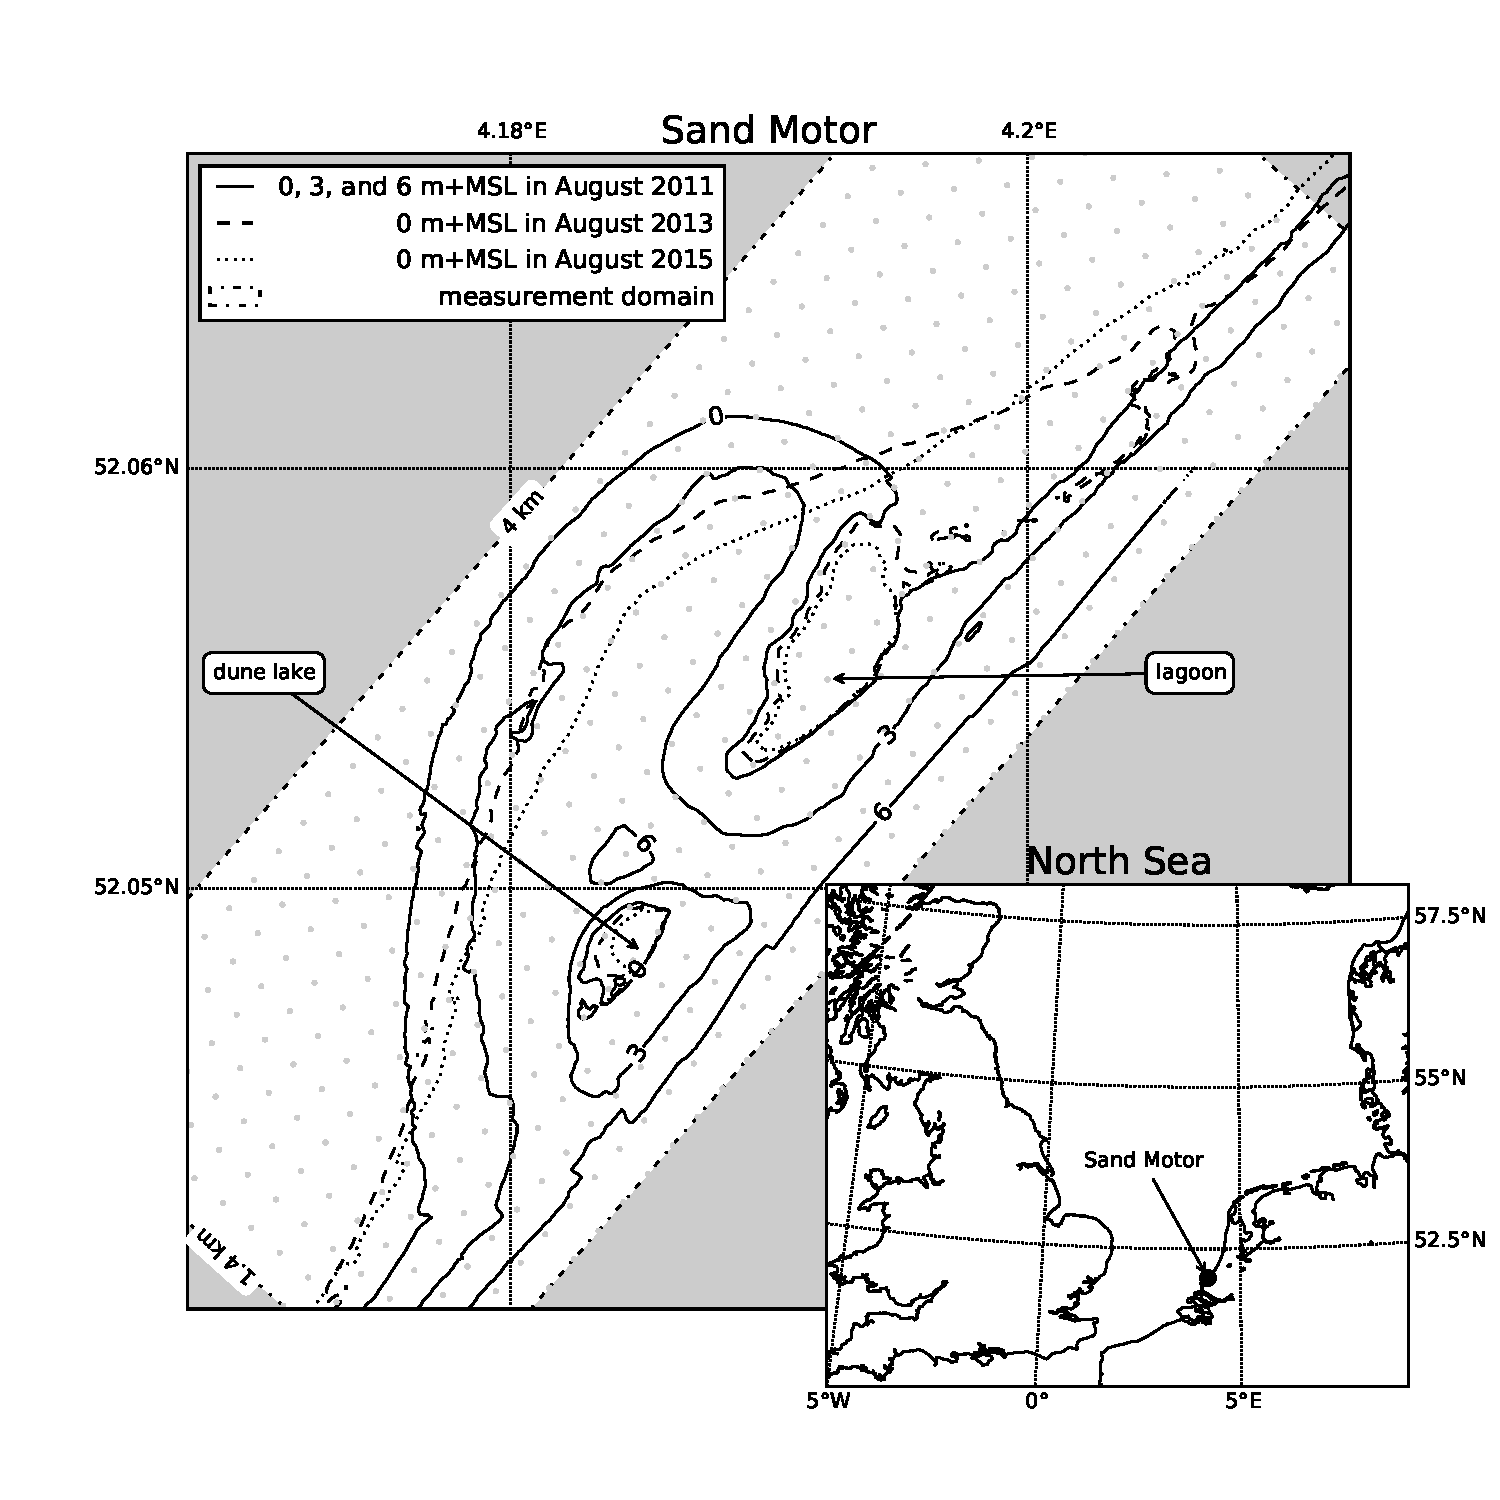
\includegraphics[width=\columnwidth]{../Figures/location_and_evolution}
  \caption{Location, orientation, appearance and evolution of the Sand
    Motor between construction in 2011 and 2015. The box indicates the
    measurement domain used in the remainder of this paper. A 100 x
    100 m grid aligned with the measurement domain is plotted in gray
    as reference.}
  \label{fig:fieldsite3}
\end{figure}

Due to natural sediment dynamics the Sand Motor distributes about 1
$\mathrm{Mm^3}$ of sand per year to the adjacent coasts (Figure
\ref{fig:fieldsite3}). The majority of this sand volume is transported
by tides and waves. However, the Sand Motor is constructed up to 5
m+MSL and locally up to 7 m+MSL, which is in either case well above
the maximum surge level of 3 m+MSL (Figure
\ref{fig:boundaryconditions}c). Therefore, the majority of the Sand
Motor area is uniquely shaped by wind.

The Sand Motor comprises both a dune lake and a lagoon that act as
large traps for aeolian sediment (Figure \ref{fig:fieldsite3}). The
lagoon is affected by tidal forcing, although the tidal amplitude
quickly diminished over time as the entry channel elongated. The tidal
range of about 2 m that is present at the Sand Motor periphery (Figure
\ref{fig:boundaryconditions}c), is nowadays damped to less than 20 cm
inside the lagoon \citep{deVries2015}. Consequently, the tidal
currents at the closed end of the lagoon, where most aeolian sediment
is trapped, are negligible.

%Sand used for construction of the Sand Motor is obtained from an
%offshore borrowing pit in the North Sea. The sand is predominantly
%Holocene sand with a significant amount of fines. The median grain
%size is slightly coarser than found originally along the Delfland
%coast. Apart from sand fractions, the sediment contains a large amount
%of shells, shell fractions, some pebbles and cobbles and an occasional
%fraction of a mammoth bone.

%\begin{figure}
%  \centering
%  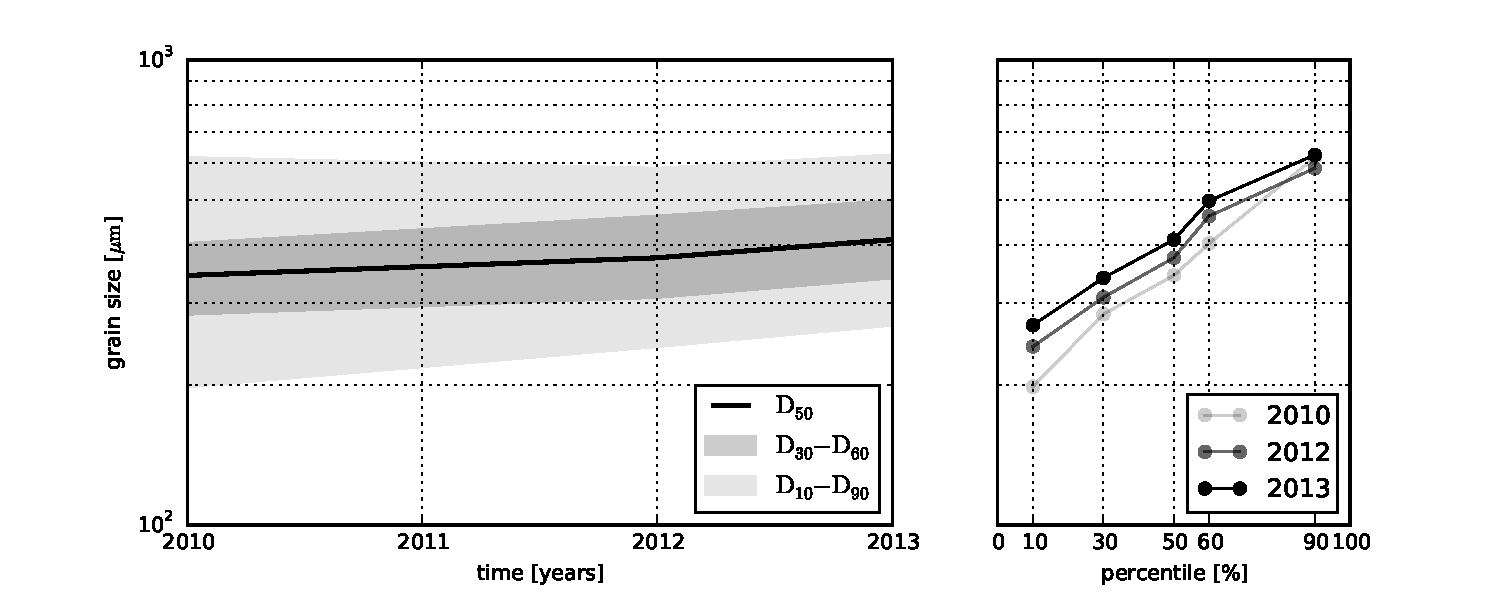
\includegraphics[width=\columnwidth]{../Figures/grainsize}
%  \caption{Evolution of the grain size distribution at the dry beach
%    since 2010, prior to construction of the Sand Motor
%    \citep{ImaresSamples}. Left panel: time series of median grain
%    size. Right panel: grain size distributions.}
%  \label{fig:grainsize}
%\end{figure}

The dominant wind direction at the Sand Motor is south to southwest
(Figure \ref{fig:boundaryconditions}a). However, during storm
conditions the wind direction tends to be southwest to
northwest. During extreme storm conditions the wind direction tends to
be northwest. Northwesterly storms are typically accompanied by
significant surges as the fetch is virtually unbounded to the
northwest, while surges from the southwest are limited due to the
presence of the narrowing of the North Sea at the Strait of Dover
(Figure \ref{fig:fieldsite3}, inset).

\begin{figure}
  \centering
  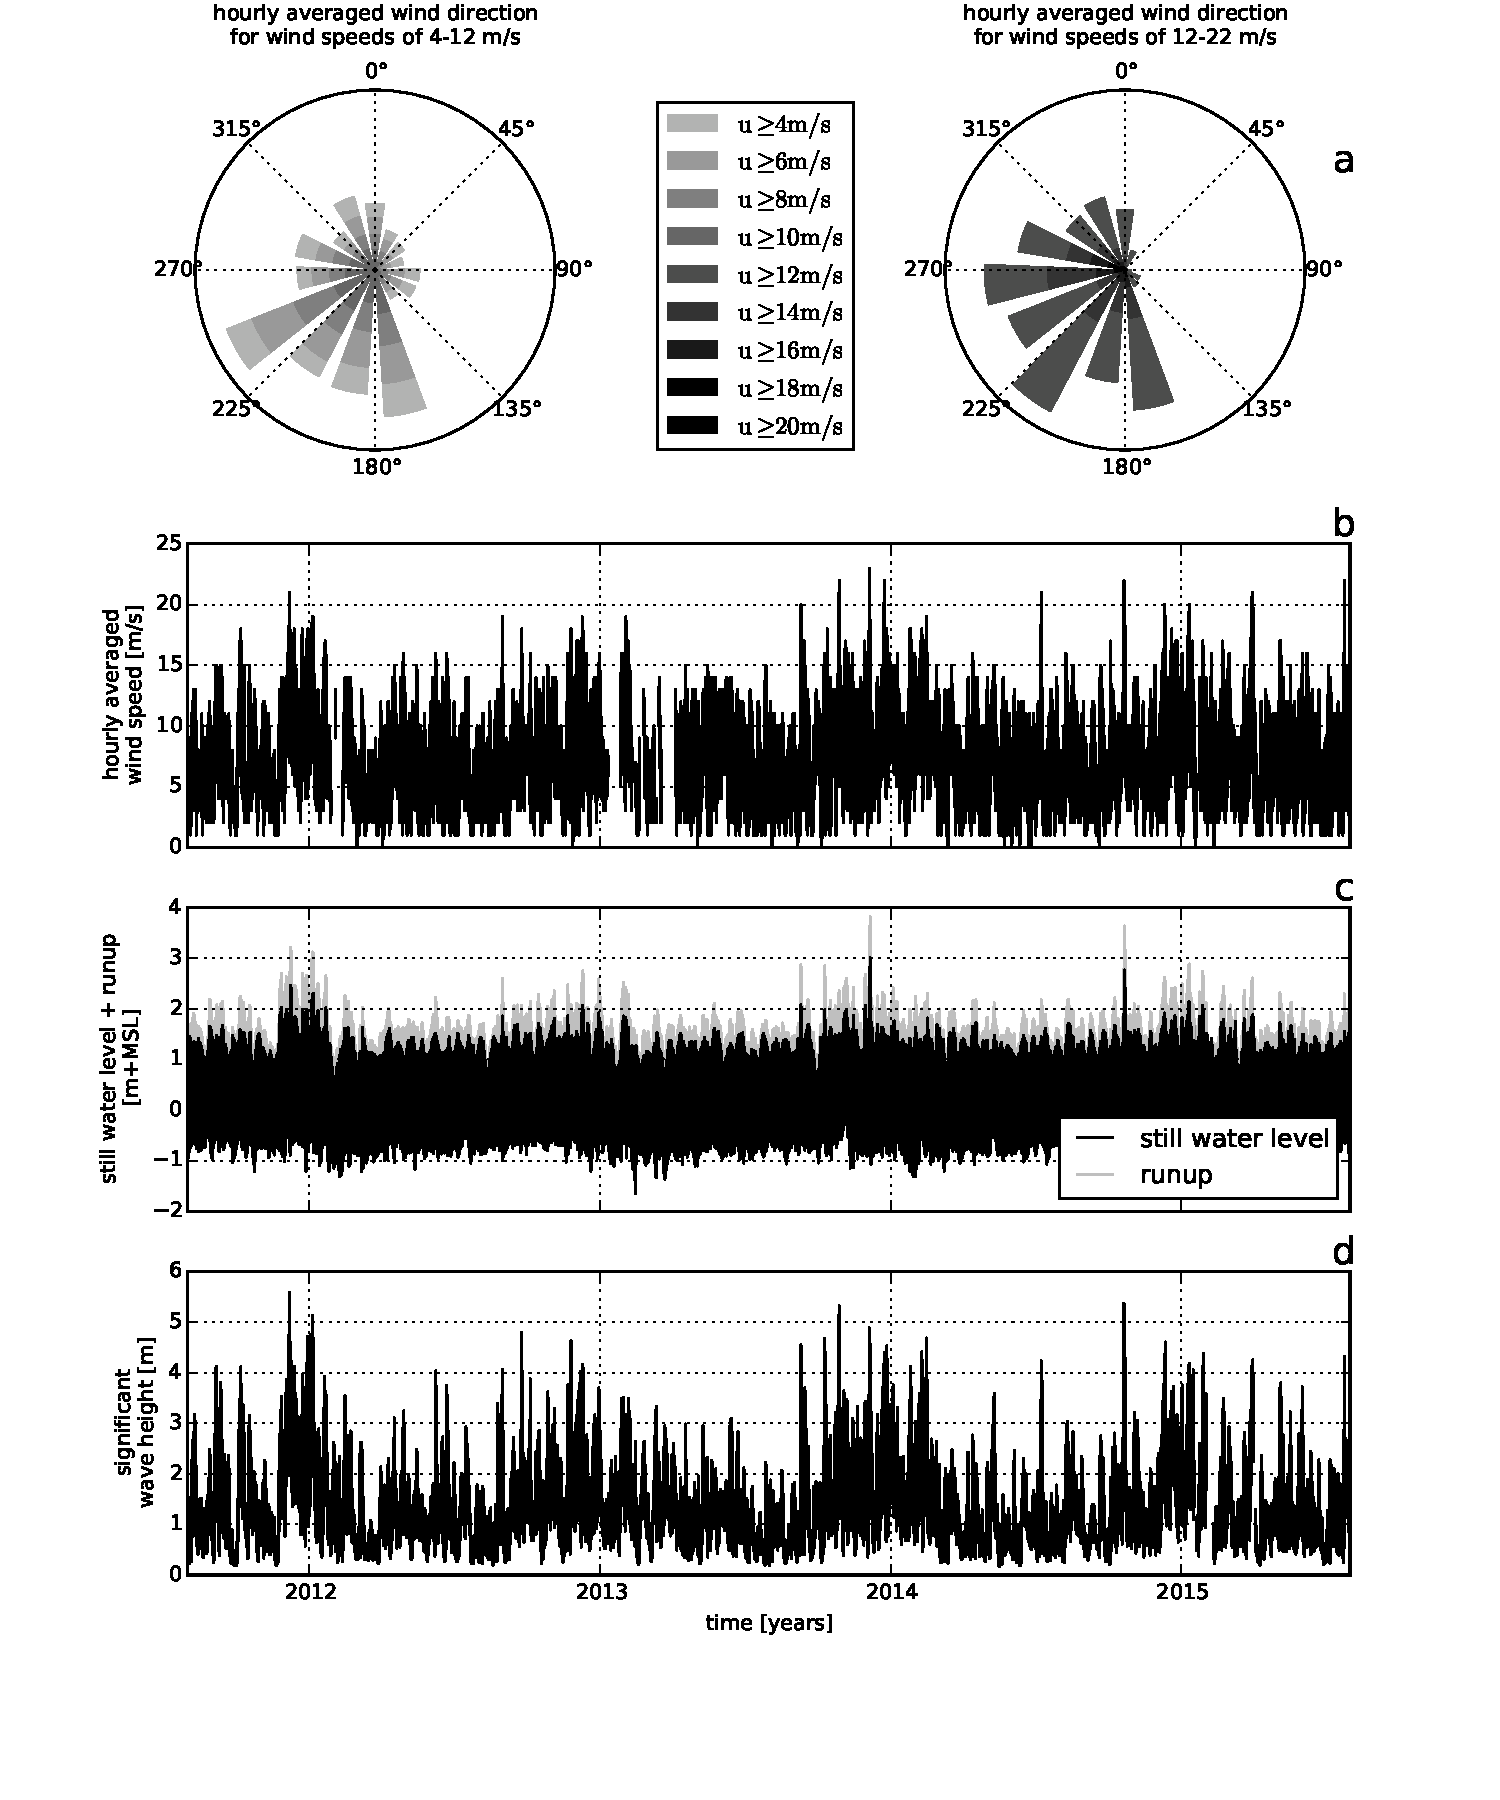
\includegraphics[width=\columnwidth]{../Figures/boundaryconditions}
  \caption{Wind and hydrodynamic time series from 2011 to 2015. Hourly
    averaged wind speeds and directions are obtained from the KNMI
    meteorological station in Hoek van Holland (upper
    panels). Offshore still water levels, wave heights and wave
    periods are obtained from the Europlatform (lower panels). Runup
    levels are estimated following \citet{Stockdon2006}.}
  \label{fig:boundaryconditions}
\end{figure}

%\section{Sediment transport capacity}
%\label{sec:transport_capacity}
%
%\begin{figure}
%  \centering
%  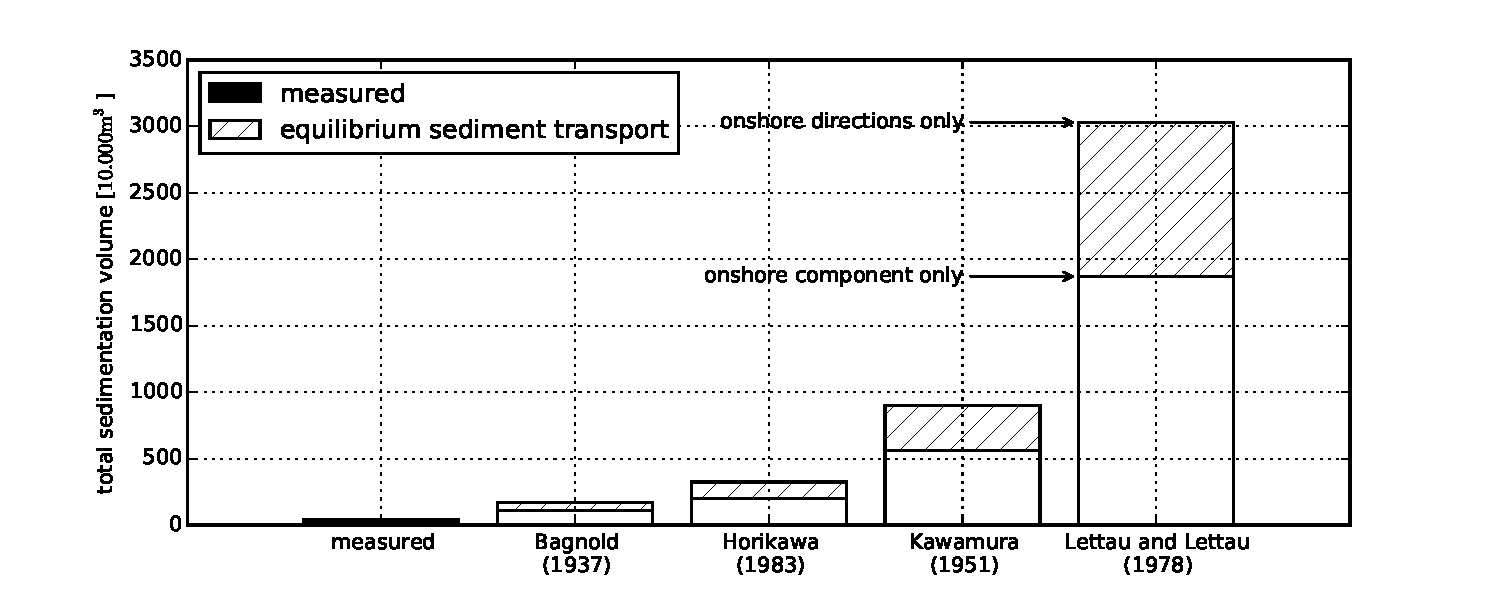
\includegraphics[width=\columnwidth]{../Figures/transport_models}
%  \caption{Comparison of the cumulative aeolian sediment transport
%    capacity according to a selection of equilibrium sediment
%    transport formulations and measured total sedimentation in the
%    Sand Motor region (upper panel). The sediment transport capacity
%    is based on an hourly averaged wind speed and direction time
%    series from September 1, 2011 until September 1, 2015. Offshore
%    wind directions are discarded. For the upper boundary of each
%    estimate all wind directions are weighted equally. For the lower
%    boundary of each estimate the wind directions are weighted
%    according to the magnitude of the onshore component. All
%    formulations overestimate the measured sedimentation volume
%    significantly. The \textsc{AeoLiS} model uses the formulation from
%    \citet{Bagnold1937a} and therefore produces comparable results if
%    all availability limiting processes are disabled (lower
%    panel). The shaded area in the lower panel is a detailed view on
%    the shaded area in the upper panel.}
%  \label{fig:models}
%\end{figure}
%
%The Sand Motor is an availability-limited system as measured aeolian
%sediment transport rates are consistently lower than the sediment
%transport capacity. The sediment transport capacity is described by
%equilibrium sediment transport formulations. Figure \ref{fig:models}
%(upper panel) presents an overview of the cumulative sediment
%transport capacity (or potential sediment accumulation) at the Sand
%Motor over the period between September 1, 2011 and September 1, 2015
%according to a selection of equilibrium sediment transport
%formulations. The cumulative sediment transport capacity $Q$
%[$\mathrm{m^3}$] is estimated based on hourly averaged time series of
%the wind speed $u_z$ [m/s] and direction $\theta_u$ [$^{\circ}$]
%obtained from the KNMI meteorological station in Hoek van Holland
%following:
%
%\begin{equation}
%  \label{eq:transport_capacity}
%  Q = \sum q \cdot f_{\theta_u} \cdot \frac{\Delta t \cdot \Delta y}{(1 - p) \cdot \rho_{\mathrm{p}}}
%\end{equation}
%
%\noindent where $\Delta t$ = 1 h, $\Delta y$ = 4 km, $p$ = 0.4,
%$\rho_{\mathrm{p}}$ = 2650 $\mathrm{kg/m^3}$, $q$ is given by the
%equilibrium sediment transport formulation (Table \ref{tab:models})
%and $f_{\theta_u}$ is a factor to account for the wind direction.
%
%\begin{table}
%  \centering
%  \caption{Equilibrium sediment transport formulations and coefficient values. 
%    Other values are $u_{\mathrm{*}} = \alpha \cdot u_z$ m/s, $u_{\mathrm{* th}} = \alpha \cdot 3.87$ m/s,
%    $\alpha = 0.058$, $\rho_{\mathrm{a}}$ = 1.25 $\mathrm{kg/m^3}$,
%    $\rho_{\mathrm{p}}$ = 2650.0 $\mathrm{kg/m^3}$, $g$ = 9.81
%    $\mathrm{m/s^2}$, $d_{\mathrm{n}}$ = 335 $\mu \mathrm{m}$, 
%    $D_{\mathrm{n}}$ = 250 $\mu \mathrm{m}$ and
%    $z$ = 10 m.}
%  \label{tab:models}
%  \begin{tabular}{lll}
%    Reference & Equation & $C$ \\
%    \hline
%    \citet{Bagnold1937a} & $q = C \frac{\rho_{\mathrm{a}}}{g} \sqrt{\frac{d_{\mathrm{n}}}{D_{\mathrm{n}}}} \left(u_{\mathrm{*}} - u_{\mathrm{* th}} \right)^3$ & 1.8 \\
%    \citet{Horikawa1983} & \multirow{2}{*}{$q = C \frac{\rho_{\mathrm{a}}}{g} \left(u_{\mathrm{*}} + u_{\mathrm{* th}} \right)^2 \left(u_{\mathrm{*}} - u_{\mathrm{* th}} \right)$} & 1.0 \\
%    \citet{Kawamura1951} &  & 2.78 \\
%    \citet{Lettau1978} & $q = C \frac{\rho_{\mathrm{a}}}{g} \sqrt{\frac{d_{\mathrm{n}}}{D_{\mathrm{n}}}} \left(u_{\mathrm{*}} - u_{\mathrm{* th}} \right) u_{\mathrm{*}}^2$ & 6.7 \\
%  \end{tabular}
%\end{table}
%
%The wind direction can be accounted for by only including the onshore
%wind component. However, given the typical Sand Motor topography,
%sediment is likely to be trapped in the dune lake and lagoon even
%without a cross-shore wind component (alongshore wind). Therefore it
%can be assumed that the onshore wind component will provide a lower
%limit of the cumulative sediment transport capacity in the Sand Motor
%region. Similarly, an upper limit can be obtained by assuming that all
%onshore wind directions contribute equally to the cumulative sediment
%transport capacity in the Sand Motor region. For the upper limit the
%factor $f_{\theta_u}$ is defined as:
%
%\begin{equation}
%  f_{\theta_u} = \left\{
%      \begin{array}{rcl}
%        1 & \mathrm{if} & \cos \left( \theta_u + 48\,^{\circ} \right) \geq 0 \\
%        0 & \mathrm{if} & \cos \left( \theta_u + 48\,^{\circ} \right) < 0 \\
%      \end{array}
%    \right.
%\end{equation}
%
%\noindent while for the lower limit the factor $f_{\theta_u}$ is defined
%as:
%
%\begin{equation}
%  f_{\theta_u} = \max \left( 0 \quad ; \quad \cos \left( \theta_u + 48\,^{\circ} \right) \right)
%\end{equation}
%
%The estimates for the sediment transport capacity show a large
%variability depending on the equilibrium sediment transport
%formulation used. The variations correspond well to the evaluations
%presented by \citet{Sherman2012} and suggest that the
%\citet{Bagnold1937a} formulation is relatively accurate. In addition,
%it is the only formulation that is suitable for multi-fraction aeolian
%sediment transport as it is derived separately for different grain
%sizes. The formulation from \citet{Bagnold1937a} is therefore selected
%for the \textsc{AeoLiS} model (Equation \ref{eq:erodep} and
%\ref{eq:equilibrium_transport}).
%
%Figure \ref{fig:models} (lower panel) shows a comparison between the
%measured sediment accumulation in the Sand Motor region, the estimates
%based on the \citet{Bagnold1937a} formulation and a preliminary
%simulation with the \textsc{AeoLiS} model in which availability
%limiting processes are disabled. The result confirms that the model
%follows the equilibrium sediment transport rate when sediment
%availability and fetch are not limited. Moreover, the result suggests
%that limitations in sediment availability reduces the sediment
%accumulation with 75\%, which is close to the upper limit of the range
%64\% -- 76\% estimated with the equilibrium sediment transport
%formulation alone.

\section{Model approach}

% link to sediment transport capacity
% link to specific results from chapter 2 for hindcast

A two-dimensional (2DH) model of the Sand Motor that includes
limitations in sediment availability is constructed and calibrated
based on four years of field measurements on wind, tides, waves and
topography. The calibrated model is used to investigate the influence
of spatiotemporal variations in aeolian sediment availability on
sediment accumulation in the Sand Motor domain.

To test that the Sand Motor mega nourishment is indeed an
availability-limited coastal system, the measured long-term sediment
accumulation volumes \citep{Hoonhout2017a} are first compared to a
reference model that assumes no limitations in sediment availability
exist.

%A numerical model of the Sand Motor region is constructed and
%calibrated for the period between September 1, 2011 and September 1,
%2015 as to investigate the influence of sediment availability on
%aeolian sediment transport rates. The sediment availability at the
%Sand Motor seems to be governed in particular by soil moisture content
%and beach armoring (Chapter \ref{ch:largescale} and
%\ref{ch:smallscale}). Therefore the calibration focuses on the drying
%rate of the soil after flooding and the sheltering of the sand surface
%by roughness elements emerging from the bed.
%
%The model presented in Chapter \ref{ch:model} is extended to obtain a
%representation of the hydrodynamic forcing that is sufficiently
%accurate for the Sand Motor hindcast. As the Sand Motor accommodates a
%dune lake, lagoon and a rapidly changing contour, large spatial
%variations in hydrodynamic forcing are present in the Sand Motor
%region. These spatial variations are largely disregarded by the model
%presented in Chapter \ref{ch:model}. Moreover, the significant
%topographic changes induced by hydrodynamic forcing are ignored.

%The calibrated model is applied to the period between September 1,
%2015 and September 1, 2016 as to test the predictive capabilities of
%the model. Testing to model on a period that has not been used for
%calibration aims at a test result independent of calibration. As
%insufficient measurements on the bed composition are available, the
%final bed composition from the calibration run is used as initial bed
%composition in the test run.

\subsection{Reference model}

\begin{figure}
  \centering
  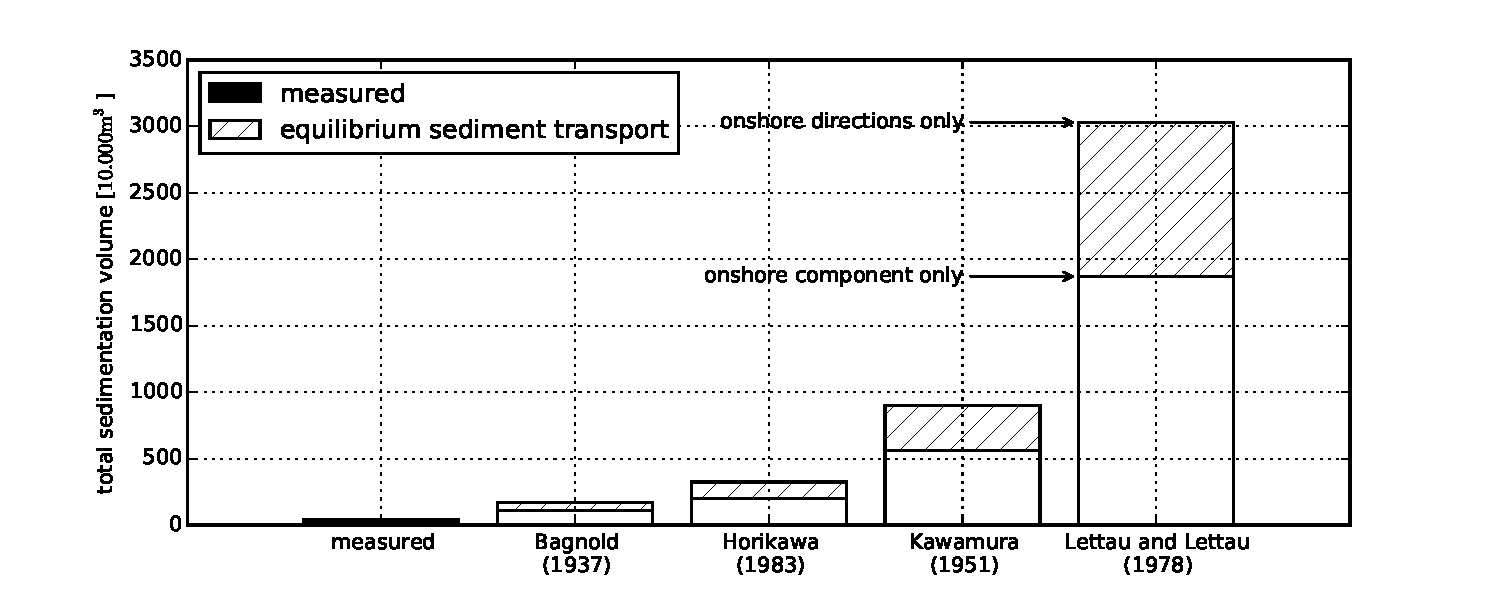
\includegraphics[width=\columnwidth]{../Figures/transport_models}
  \caption{Comparison of the cumulative wind transport capacity
    according to a selection of equilibrium sediment transport
    formulations and measured total sedimentation in the Sand Motor
    domain. The equilibrium sediment transport is based on an hourly
    averaged wind speed and direction time series from September 1,
    2011 until September 1, 2015. Offshore wind directions are
    discarded. For the upper boundary of each estimate all wind
    directions are weighted equally. For the lower boundary of each
    estimate the wind directions are weighted according to the
    magnitude of the onshore component.}
  \label{fig:models}
\end{figure}

A selection of equilibrium sediment transport formulations is used as
reference model. An equilibrium sediment transport formulation
describes the wind transport capacity in given conditions. In
conjunction with a shear velocity threshold based on only a constant
uniform median grain size, an estimate of the potential aeolian
sediment accumulation in absence of availability-limitations can be
obtained. The potential aeolian sediment accumulation or cumulative
wind transport capacity $Q$ [$\mathrm{m^3}$] in the Sand Motor domain
is estimated based on hourly averaged time series of the wind speed
$u_z$ [m/s] and direction $\theta_u$ [$^{\circ}$] obtained from the
KNMI meteorological station in Hoek van Holland following:

\begin{equation}
  \label{eq:transport_capacity}
  Q = \sum q \cdot \frac{\Delta t \cdot \Delta y}{(1 - p) \cdot \rho_{\mathrm{p}}} \cdot f_{\theta_u}
\end{equation}

\noindent where the temporal resolution $\Delta t$ = 1 h, the
alongshore span of the domain $\Delta y$ = 4 km, the porosity $p$ =
0.4, the particle density $\rho_{\mathrm{p}}$ = 2650
$\mathrm{kg/m^3}$, the sediment transport rate $q$ is given by the
equilibrium sediment transport formulation (Table \ref{tab:models})
and $f_{\theta_u}$ is a factor to account for the wind direction. The
wind direction can be accounted for by only including the onshore wind
component with respect to the original coastline orientation. However,
given the typical Sand Motor geometry (Figure \ref{fig:fieldsite3}),
sediment is likely to be trapped in the dune lake and lagoon even with
alongshore wind. Therefore it can be assumed that the onshore wind
component will provide a lower limit of the cumulative wind transport
capacity. Similarly, an upper limit can be obtained by assuming that
all onshore wind directions contribute equally to the cumulative wind
transport capacity. For the upper limit the factor $f_{\theta_u}$ is
defined as:

\begin{equation}
  f_{\theta_u} = \left\{
      \begin{array}{rcl}
        1 & \mathrm{if} & \cos \left( 312\,^{\circ} - \theta_u \right) \geq 0 \\
        0 & \mathrm{if} & \cos \left( 312\,^{\circ} - \theta_u \right) < 0 \\
      \end{array}
    \right.
\end{equation}

\noindent while for the lower limit the factor $f_{\theta_u}$ is defined
as:

\begin{equation}
  f_{\theta_u} = \max \left( 0 \quad ; \quad \cos \left( 312\,^{\circ} - \theta_u \right) \right)
\end{equation}

\noindent where $312\,^{\circ}$ accounts for orientation of the original
coastline.  Figure \ref{fig:models} presents an overview of the
cumulative wind transport capacity in the Sand Motor domain over the
period between September 1, 2011 and September 1, 2015 according to a
selection of equilibrium sediment transport formulations and in
comparison with the measured accumulation volumes. The estimates of
the wind transport capacity show a large variation between
formulations that are mainly due to the incorporation of the shear
velocity threshold. However, all formulations overestimate the
measured sediment accumulation in the Sand Motor domain with at least
a factor 3 -- 4. The large variation and consistent overestimation is
in accordance with the review of aeolian sediment transport models
presented by \citet{Sherman2012}. The consistent overestimation of the
measured sedimentation volumes in the Sand Motor domain suggest that
the Sand Motor is indeed an availability-limited coastal system.

\subsection{Schematization}

\begin{figure}
  \centering
  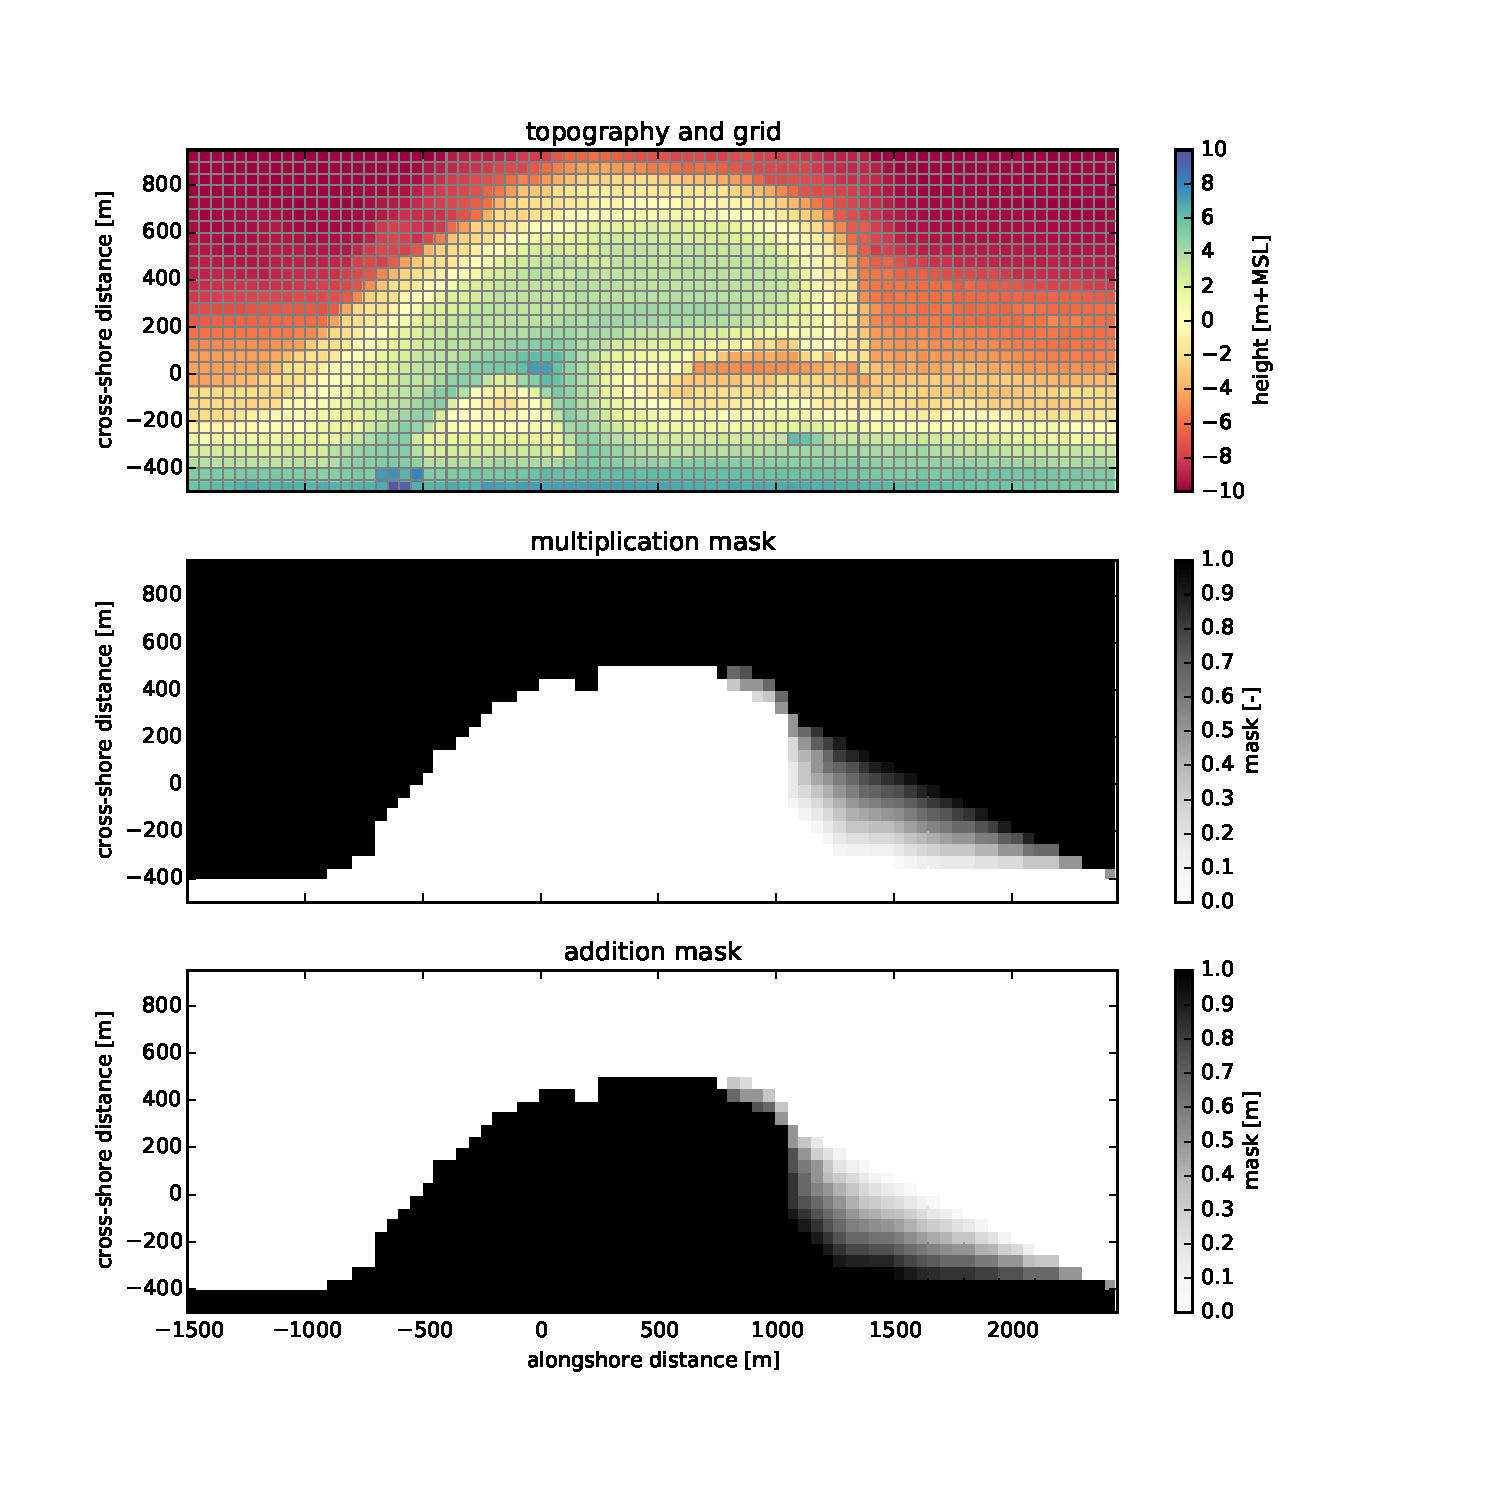
\includegraphics[width=\columnwidth]{../Figures/gridmask}
  \caption{Model grid and topography based on the topographic survey
    of August 3, 2011 (upper panel) and hydrodynamic mask used to
    limit tidal and wave motions in the dune lake and lagoon (middle
    and lower panels). Water levels and wave heights are uniformly
    imposed to the model and multiplied by the multiplication mask and
    subsequently increased with the addition mask.}
  \label{fig:gridmask}
\end{figure}

%\begin{figure}
%  \centering
%  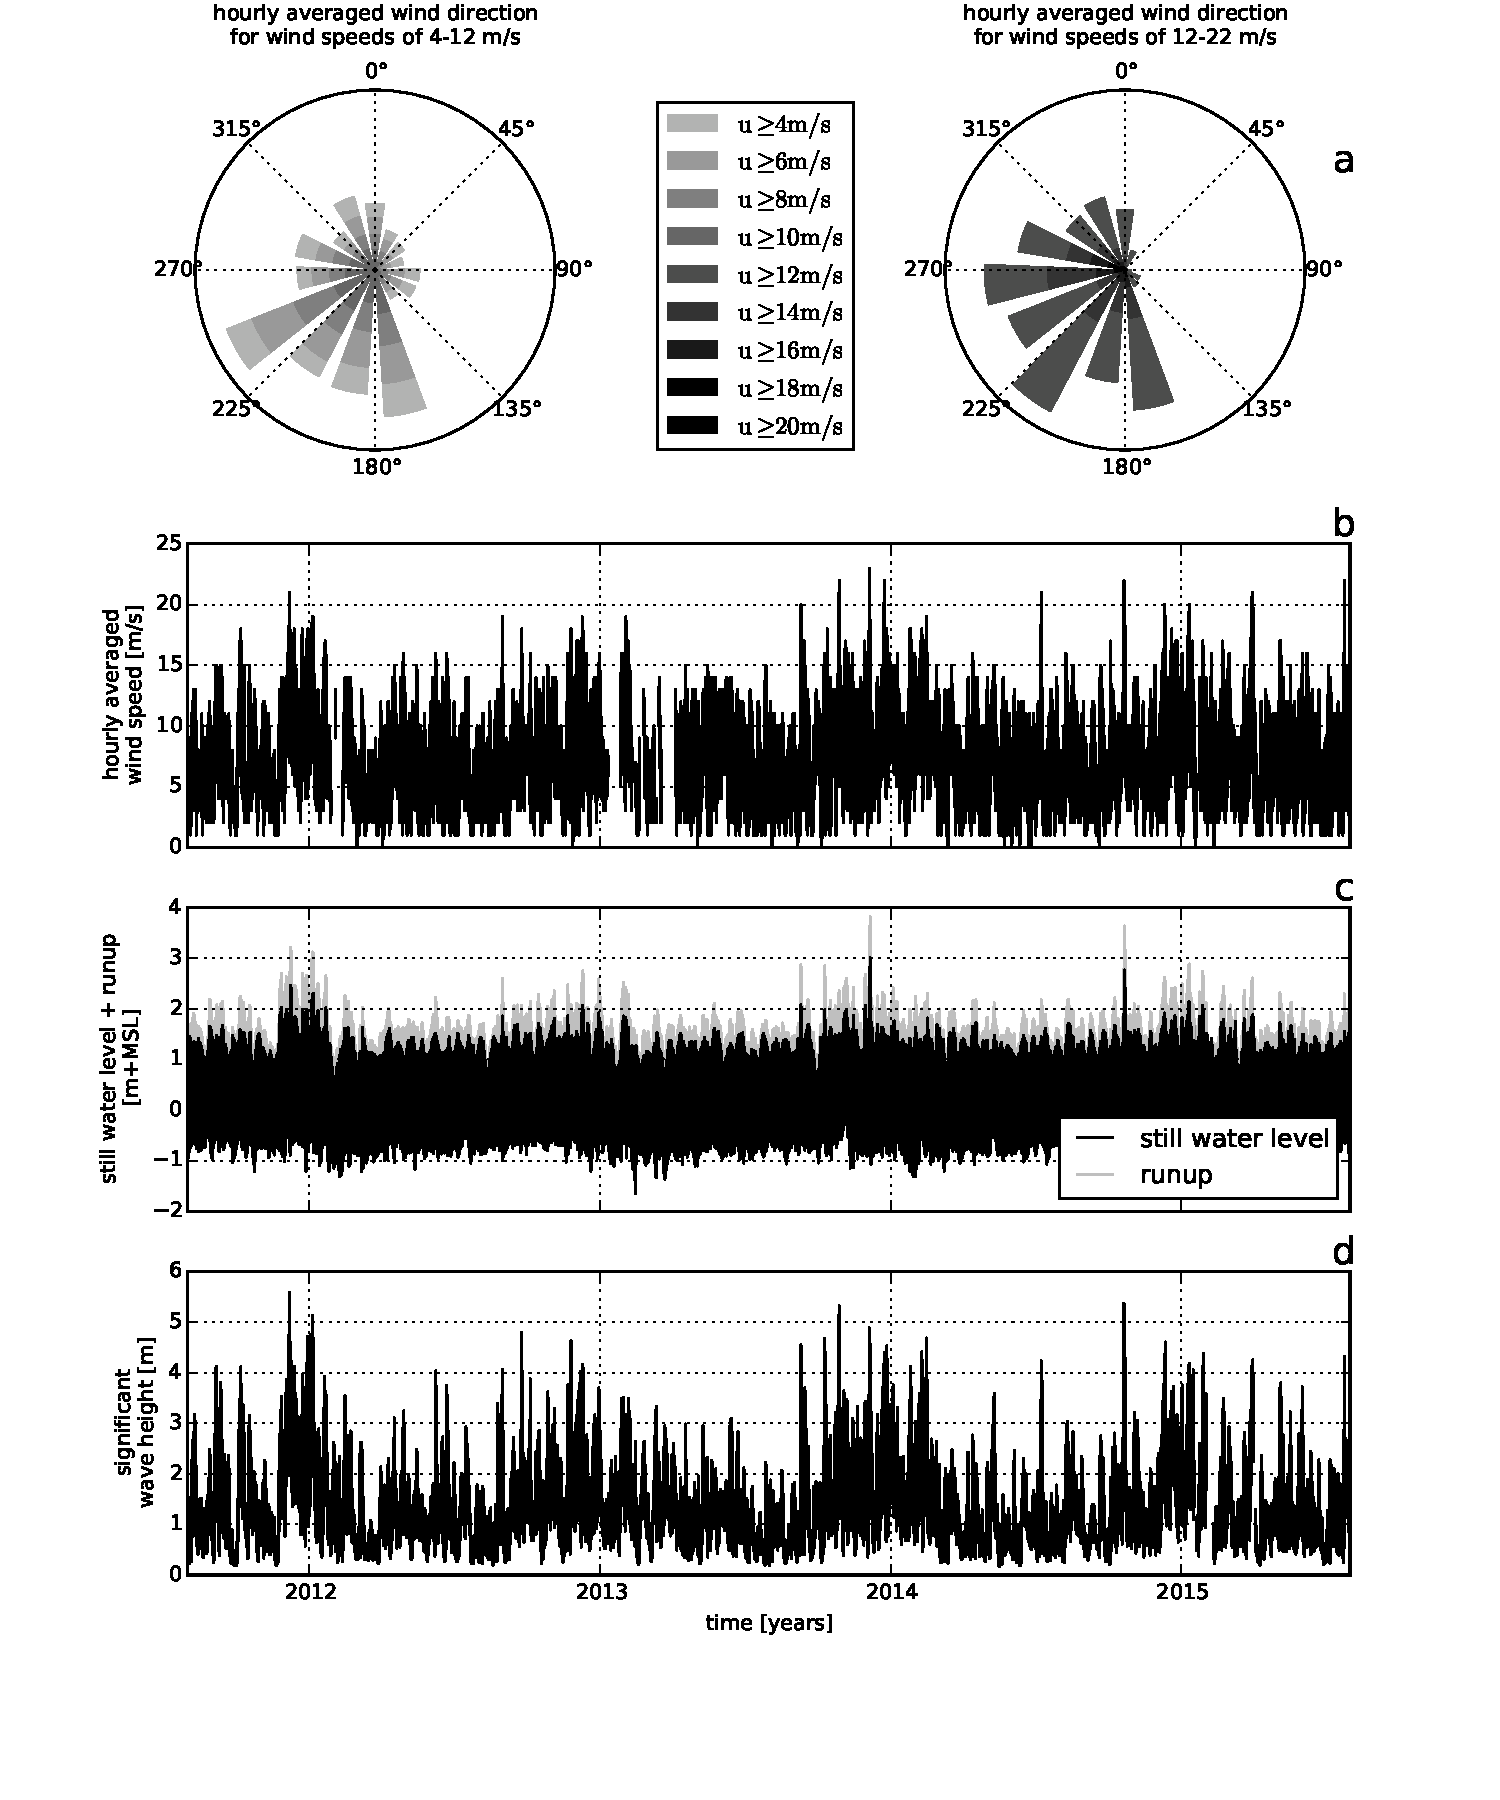
\includegraphics[width=\columnwidth]{../Figures/boundaryconditions}
%  \caption{Wind and hydrodynamic boundary conditions imposed to the
%    model. Hourly averaged wind speeds and directions are obtained
%    from the KNMI meteorological station in Hoek van Holland (upper
%    panels). Offshore still water levels, wave heights and wave
%    periods are obtained from the Europlatform (lower panels). Runup
%    levels are estimated following \citet{Stockdon2006}.}
%  \label{fig:boundaryconditions}
%\end{figure}

% topography and grid
A two-dimensional (2DH) aeolian sediment availability and transport
model for the Sand Motor mega nourishment is constructed for the four
years between September 1, 2011 and September 1, 2015, which is
shortly after the nourishment was placed. The model's topography and
grid are based on the measured topographies of August 3, 2011 and
later. The topographies are rotated $48\,^{\circ}$ and interpolated to
a 50 x 50 m grid spanning 1.5 km cross-shore and 4 km alongshore with
respect to the original coastline, not including the dunes (Figure
\ref{fig:gridmask}, upper panel).

% boundary conditions
Four years of hourly wind speed and direction data measured at 10 m
above the bed is obtained from the KNMI meteorological station at Hoek
van Holland (Figure \ref{fig:boundaryconditions}a,b). Hourly offshore
water levels and wave heights are obtained from the Europlatform for
the same period (Figure \ref{fig:boundaryconditions}c,d).

% grain size and shells, layers and layer thickness
An average lognormal grain size distribution with a median diameter
$d_{50} = 335 ~ \mu \mathrm{m}$ is used as measured at the Sand Motor
field site. The sand fractions cover a range from 0.1 to 2 mm. The
amount of shells and other roughness elements in the originally
nourished sand is estimated to be 5\%. The estimate is based on three
sediment samples obtained from the field site 0.5 m below the bed
surface. Additional fractions ranging from 2 to 32 mm are added
according to a lognormal distribution to account for the presence of
roughness elements in the bed. The grain size distribution is used to
populate the initial bed that consists of 10 bed composition layers
with a thickness of 1 cm each.

% timestep and scheme
The hindcast aims at the large scale and long term sedimentation
volumes as presented by \citet{Hoonhout2016a}. Therefore an efficient,
but diffusive, implicit Euler Backward scheme with a timestep of 1 h
is used that does not resolve high frequency variations in wind or
sediment transport. Consequently, the model produces smooth solutions
that describe hourly steady states based on the instantaneous average
wind speed and sediment availability.

% equilibrium sediment transport formulation

\begin{table}
  \centering
  \caption{Equilibrium sediment transport formulations, coefficient
    values* and the ratio between measurements and model results.}
  \label{tab:models}
  \begin{tabular}{llll}
    Reference & Equation & $C$ & Ratio \\
    \hline
    \citet{Bagnold1937a} & $q = C \frac{\rho_{\mathrm{a}}}{g} \sqrt{\frac{d_{\mathrm{n}}}{D_{\mathrm{n}}}} \left(u_{\mathrm{*}} - u_{\mathrm{* th}} \right)^3$ & 1.8 & 3 -- 4 \\
    \citet{Horikawa1983} & \multirow{2}{*}{$q = C \frac{\rho_{\mathrm{a}}}{g} \left(u_{\mathrm{*}} + u_{\mathrm{* th}} \right)^2 \left(u_{\mathrm{*}} - u_{\mathrm{* th}} \right)$} & 1.0 & 5 -- 8 \\
    \citet{Kawamura1951} &  & 2.78 & 14 -- 22 \\
    \citet{Lettau1978} & $q = C \frac{\rho_{\mathrm{a}}}{g} \sqrt{\frac{d_{\mathrm{n}}}{D_{\mathrm{n}}}} \left(u_{\mathrm{*}} - u_{\mathrm{* th}} \right) u_{\mathrm{*}}^2$ & 6.7 & 46 -- 75 \\
  \end{tabular}

  \footnotesize{
    \begin{enumerate}[{*}]
    \item Other values are the shear velocity
      $u_{\mathrm{*}} = \alpha \cdot u_z$ m/s, the shear velocity
      threshold $u_{\mathrm{* th}} = \alpha \cdot 3.87$ m/s, the
      conversion factor from free-flow wind velocity to shear velocity
      $\alpha = 0.058$, the air density $\rho_{\mathrm{a}}$ = 1.25
      $\mathrm{kg/m^3}$, the particle density $\rho_{\mathrm{p}}$ =
      2650.0 $\mathrm{kg/m^3}$, the gravitational constant $g$ = 9.81
      $\mathrm{m/s^2}$, the nominal grain size $d_{\mathrm{n}}$ = 335
      $\mu \mathrm{m}$, a reference grain size $D_{\mathrm{n}}$ = 250
      $\mu \mathrm{m}$ and the height above the bed of the wind
      measurement $z$ = 10 m.
    \end{enumerate}
  }
\end{table}

\citet{Bagnold1937a} is selected as equilibrium sediment transport
formulation as it is derived separately for different grain sizes and
therefore suitable for multi-fraction aeolian sediment
transport. Alternative formulations (Table \ref{tab:models}) are
derived for wider grain size distributions that do not necessarily
result in a monotonic relation between the grain size and the sediment
transport rate \citep[e.g.][]{Kawamura1951, Horikawa1983}. Such
non-monotonic relation is unrealistic in a multi-fraction context as
it would result in a preference to transport both fine sediment and
large elements that are considered non-erodible. Moreover, the
formulation of \citet{Bagnold1937a} overestimates the measured aeolian
sediment transport rates in the Sand Motor domain less compared to
alternative formulations (Table \ref{tab:models}, rightmost column).

% masks
Water levels and wave heights are initially uniformly imposed to the
model. Consequently, the tidal range, mean water level and wave
heights that are present at the Sand Motor periphery are also present
in the dune lake and lagoon. In reality the tidal range and wave
heights in the dune lake and lagoon are much lower, while the mean
water level in the dune lake and lagoon is elevated compared to mean
sea level \citep{deVries2015}. To account for these spatial
differences in hydrodynamics a hydrodynamic mask is applied (Figure
\ref{fig:gridmask}, middle and lower panel; Appendix \ref{apx:mask})

% BMI
Subtidal changes in topography are not simulated by the model. The
subtidal changes can be important to aeolian sediment transport as the
location and size of aeolian sediment erosion and deposition areas
might change. To account for these changes, measured topographies are
imposed to the model through a Basic Model Interface
\citep[BMI,][Appendix \ref{apx:bmi}]{Peckham2013}.

All measured topographies in the period between September 1, 2011 and
September 1, 2015 are linearly interpolated in time as to obtain daily
updates of the Sand Motor's topography. The hydrodynamic mask is
updated along with the topography. The presented aeolian sediment
transport rates are based on the time-integrated entrainment and
deposition rates that are computed by the model rather than
differences in topography.

\subsection{Calibration}

The model is calibrated on the shape of roughness elements that emerge
from the bed and shelter the sand surface from wind erosion, the
drying rate of the soil and the time needed for the sediment transport
to adapt to changing wind conditions. These processes are represented
in the model by parameters for which data or literature can only
provide approximate values:

\begin{enumerate}
\item $\sigma$, as used in the formulation of \citet[][Equation
  \ref{eq:raupach}]{Raupach1993}, is the ratio between the basal and
  frontal area of the roughness elements that constitute the beach
  armor layer.
\item $T_{\mathrm{dry}}$ is the time scale at which the beach dries
  out after flooding (Equation \ref{eq:apx_drying}). It represents the
  time in which the soil moisture content halves in case the beach is
  not inundated and no evaporation occurs.
\item $T$ is the adaptation time scale in the right-hand side of the
  advection equation (Equation \ref{eq:erodep}). It represents the
  time scale to which the sediment transport adapts to variations in
  the wind conditions and sediment availability.
\end{enumerate}

% Wind tunnel experiments presented by \citet{McKennaNeuman2012}
% provide leads on appropriate values for $\sigma$. The wind tunnel
% experiments investigated the influence of a beach armor layer,
% consisting of shells and shell fragments, on aeolian sediment
% transport. The results were used to derive optimal values for the
% parameters $\sigma$ and $\beta$ (Equation \ref{eq:raupach}).

The implementation of roughness elements is characterized by three
calibration parameters: $m$, $\beta$ and $\sigma$ (Equation
\ref{eq:raupach2}). $m$ is a factor to account for the difference
between the mean and maximum shear stress and is usually chosen as 0.5
for field applications \citep{Raupach1993,
  McKennaNeuman2012}. Numerically it is irrelevant if $\beta$ or
$\sigma$ is calibrated as they only appear as a ratio
$\frac{\beta}{\sigma}$ in the model implementation. As $\beta$ is the
ratio between the drag coefficient of the roughness elements alone and
the drag coefficient of the unarmored sandy bed, the value can be
assumed to be reasonably generic. In contrast, $\sigma$ depends on the
shape and protrusion of the roughness elements and therefore depends
on the field site and varies in time. For example, a spherical object
placed on top of the bed would be represented by $\sigma = 1$, while a
spherical object protruding halfway through the bed (hemisphere) would
be represented by $\sigma = 2$. Consequently, calibration of $\sigma$
seems to be preferable as it is less certain. Wind tunnel experiments
presented by \citet{McKennaNeuman2012} investigated the influence of a
lag deposits, consisting of shells and shell fragments, on aeolian
sediment transport. Values for the calibration coefficients $m$ and
$\beta$ were found to be 0.5 and 130 respectively and are adopted for
the Sand Motor hindcast. An optimal average value for $\sigma$ is
obtained by systematic variation between 2 and 20.

The drying rate of the beach ($T_{\mathrm{dry}}$) depends on many
factors, like grain size, soil moisture content, groundwater level,
wind speed and solar radiation. The use of a single time scale as
aggregate for these processes is an oversimplification of
reality. Therefore a wide range of parameter values is covered in the
calibration. $T_{\mathrm{dry}}$ is varied between 0.1 and 10 hours
where the former results in virtually instant drying and the latter
results in an intertidal beach that is permanently too moist for
aeolian sediment transport to be initiated.

The adaptation time scale ($T$), that represents the swiftness of
aeolian sediment transport to adapt to changing wind conditions, is in
the order of seconds \citep{DavidsonArnott2008, deVries2014a}. As the
model time step is orders of magnitude larger, the model effectively
solves steady states and the value for $T$ will not affect temporal
variations in sediment transport. However, the adaptation time scale
also affects the development of the saltation cascade in
space. Sediment transport increases in downwind direction from a
zero-flux boundary, like the water line in case of onshore wind, with
a rate that is governed by the value of $T$. Consequently, $T$
influences the width of the source area in case of abundant sediment
availability. $T$ is varied between 1 and 10 seconds.

\begin{figure}
  \centering
  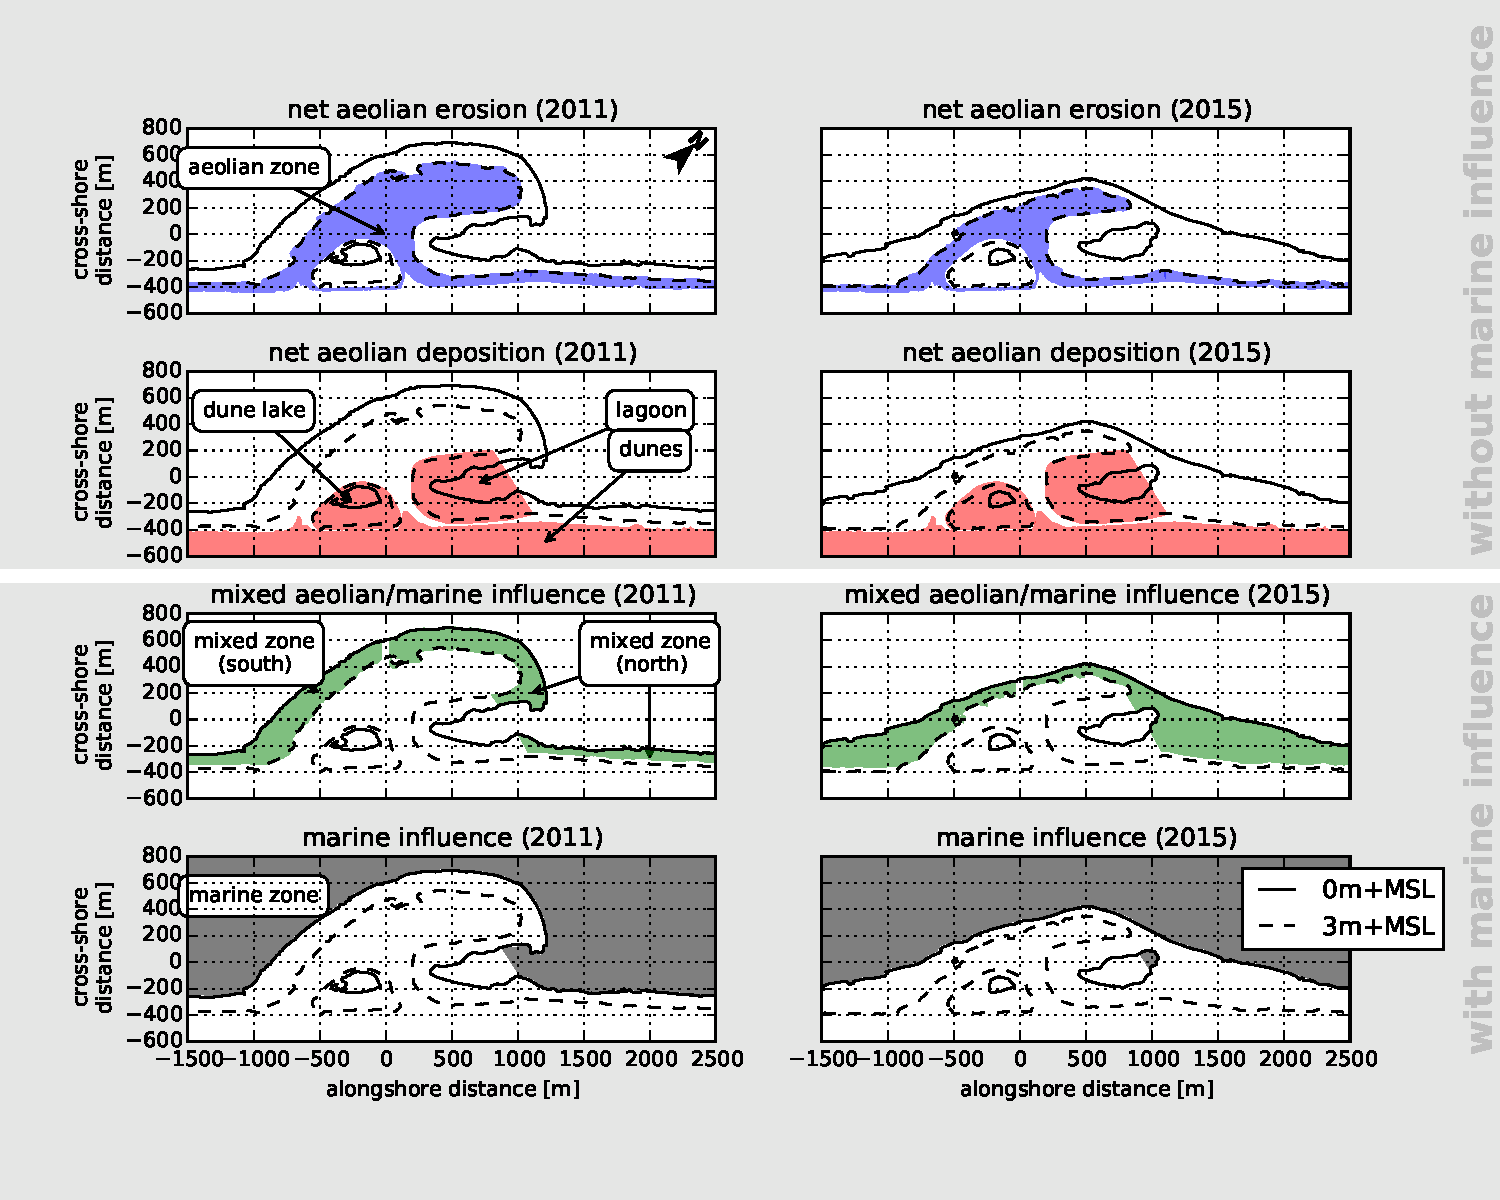
\includegraphics[width=\columnwidth]{../Figures/decomposition}
  \caption{Zonation of the Sand Motor domain into zones with net
    aeolian erosion and no marine influence, net aeolian deposition
    and no marine influence, mixed aeolian/marine influence and marine
    influence. Zonation is based on the 0, 3 and 5 m+MSL contour lines
    that roughly correspond with the mean water level, maximum runup
    level or berm edge and the dune foot respectively. Left panels:
    2011. Right panels: 2015. Source: \citet{Hoonhout2017a}.}
  \label{fig:decomposition2}
\end{figure}

The calibration is performed based on the bi-monthly erosion and
deposition volumes as measured in the Sand Motor domain
\citep{Hoonhout2017a}. The erosion and deposition volumes are
determined within seven predefined zones (Figure
\ref{fig:decomposition2}) that aim to separate areas with marine
influences from areas without marine influences, and separate areas
with net aeolian erosion from areas with net aeolian deposition. The
zonation is based on the 0, 3 and 5 m+MSL contour lines that roughly
correspond with the mean water level, maximum runup level or berm edge
and the dune foot respectively. The average $\mathrm{R^2}$ value of
the time series for erosion and deposition is used as benchmark. The
$\mathrm{R^2}$ value represents the fraction of explained variance and
is defined as:

\begin{equation}
  \label{eq:r2}
  R^2 = \frac{\sum_n \left[ V^n_{\mathrm{measured}} - V^n_{\mathrm{model}} \right]^2}{\sum_n \left[ V^n_{\mathrm{measured}} - \overline{V^n_{\mathrm{measured}}} \right]^2}
\end{equation}

\noindent where $V^n$ is the measured or modeled sediment volume in
time period $n$. The overbar denotes time-averaging. In addition the
root-mean-square error (RMSE) is presented as absolute measure for the
model accuracy, which is defined as:

\begin{equation}
  \label{eq:rmse}
  RMSE = \sqrt{\sum_n \left[ V^n_{\mathrm{measured}} - V^n_{\mathrm{model}} \right]^2}
\end{equation}

\noindent The calibration itself is performed in three steps:

\begin{enumerate}
\item A coarse calibration on $\sigma$ and $T_{\mathrm{dry}}$.
\item A calibration on $T$ using the provisional optimal settings for
  $\sigma$ and $T_{\mathrm{dry}}$.
\item A fine calibration on $\sigma$ and $T_{\mathrm{dry}}$ using the
  optimal setting for $T$.
\end{enumerate}

\section{Results}

The optimal model settings were chosen from 150 realizations (Figure
\ref{fig:calibration}). The optimal realization has an $\mathrm{R^2}$
value of 0.92 and a RMSE of $3 \cdot 10^4 ~ \mathrm{m^3}$.
\mrq{4.1} % (Table \ref{tab:stats}).
The corresponding optimal parameter settings are found to be
$\sigma = 9.2$, $T_{\mathrm{dry}} = 2$ h and $T$ = 1 s. These
settings were ultimately selected from a cluster of realizations with
comparable $\mathrm{R^2}$ values based on the relative sediment supply
from the mixed zones (Figure \ref{fig:decomposition2}, third row) at
the end of the simulation. An overview of all model settings for the
calibrated model is given in Appendix \ref{apx:modelsettings}.

%\begin{table}
%  \centering
%  \caption{Performance statistics of the calibrated Sand Motor model
%    for the calibration and test period.}
%  \label{tab:stats}
%  \begin{tabular}{lcccc}
%    Period & \multicolumn{2}{c}{RMSE} & $\mathrm{R}^2$ & rel. supply from \\
%    ~ & [$\mathrm{m^3}$] & [\%] & [-] & intertidal beach \\
%    \hline
%    2011 -- 2015 & $2.9 \cdot 10^4$ & 7.2 & 0.93 & 56\% \\
%    2015 -- 2016 & $2.9 \cdot 10^4$ & 7.2 & 0.93 & 56\% \\
%  \end{tabular}
%\end{table}

\begin{figure}
  \centering
  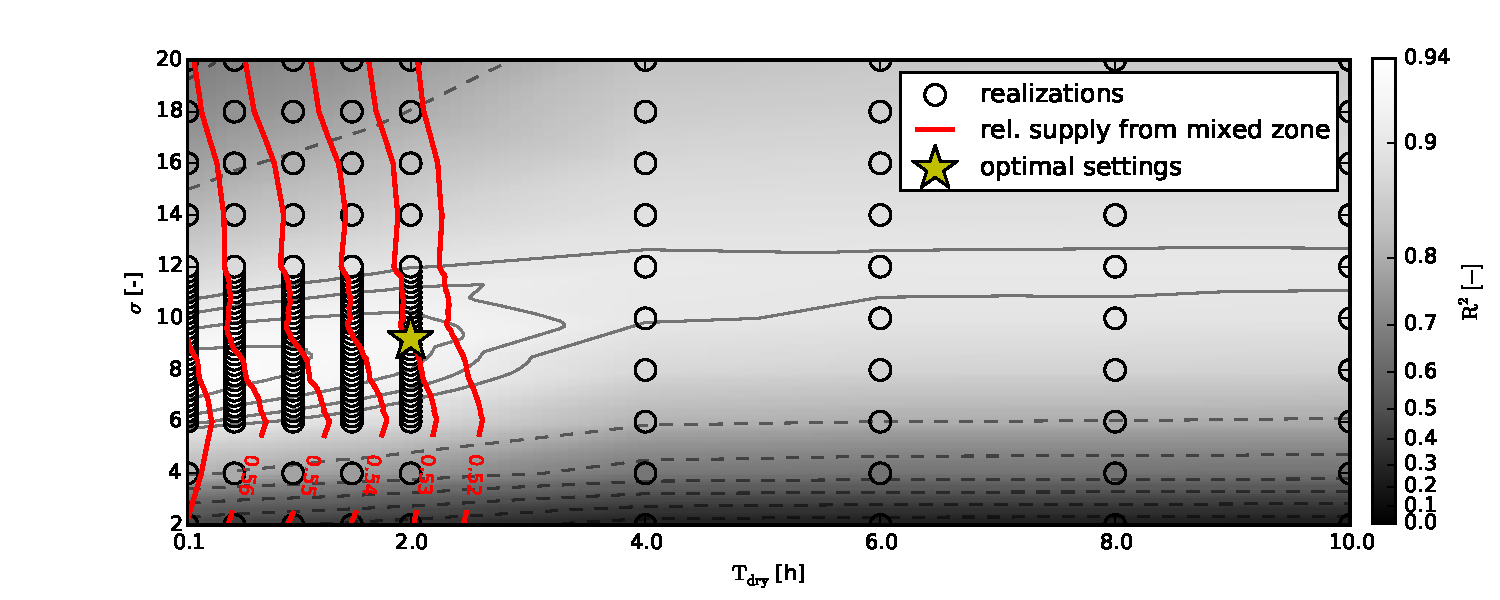
\includegraphics[width=\columnwidth]{../Figures/calibration}
  \caption{Systematic variation of calibration parameters $\sigma$ and
    $T_{\mathrm{dry}}$ with $T$ = 1 s. The circles indicate the
    realizations made. The colored background depicts a linear
    interpolation of the $\mathrm{R^2}$ values with respect to the
    data presented in Figure \ref{fig:netvolumechange}. The solid
    isolines depict $\mathrm{R}^2$ values from 0.90 to 0.93, while the
    dashed isolines depict $\mathrm{R}^2$ values from 0.0 to 0.9. The
    red lines depict the relative supply from the mixed zones ranging
    from 52\% to 57\%. The yellow star indicates the optimal value
    model settings.}
  \label{fig:calibration}
\end{figure}


\begin{figure}
  \centering
  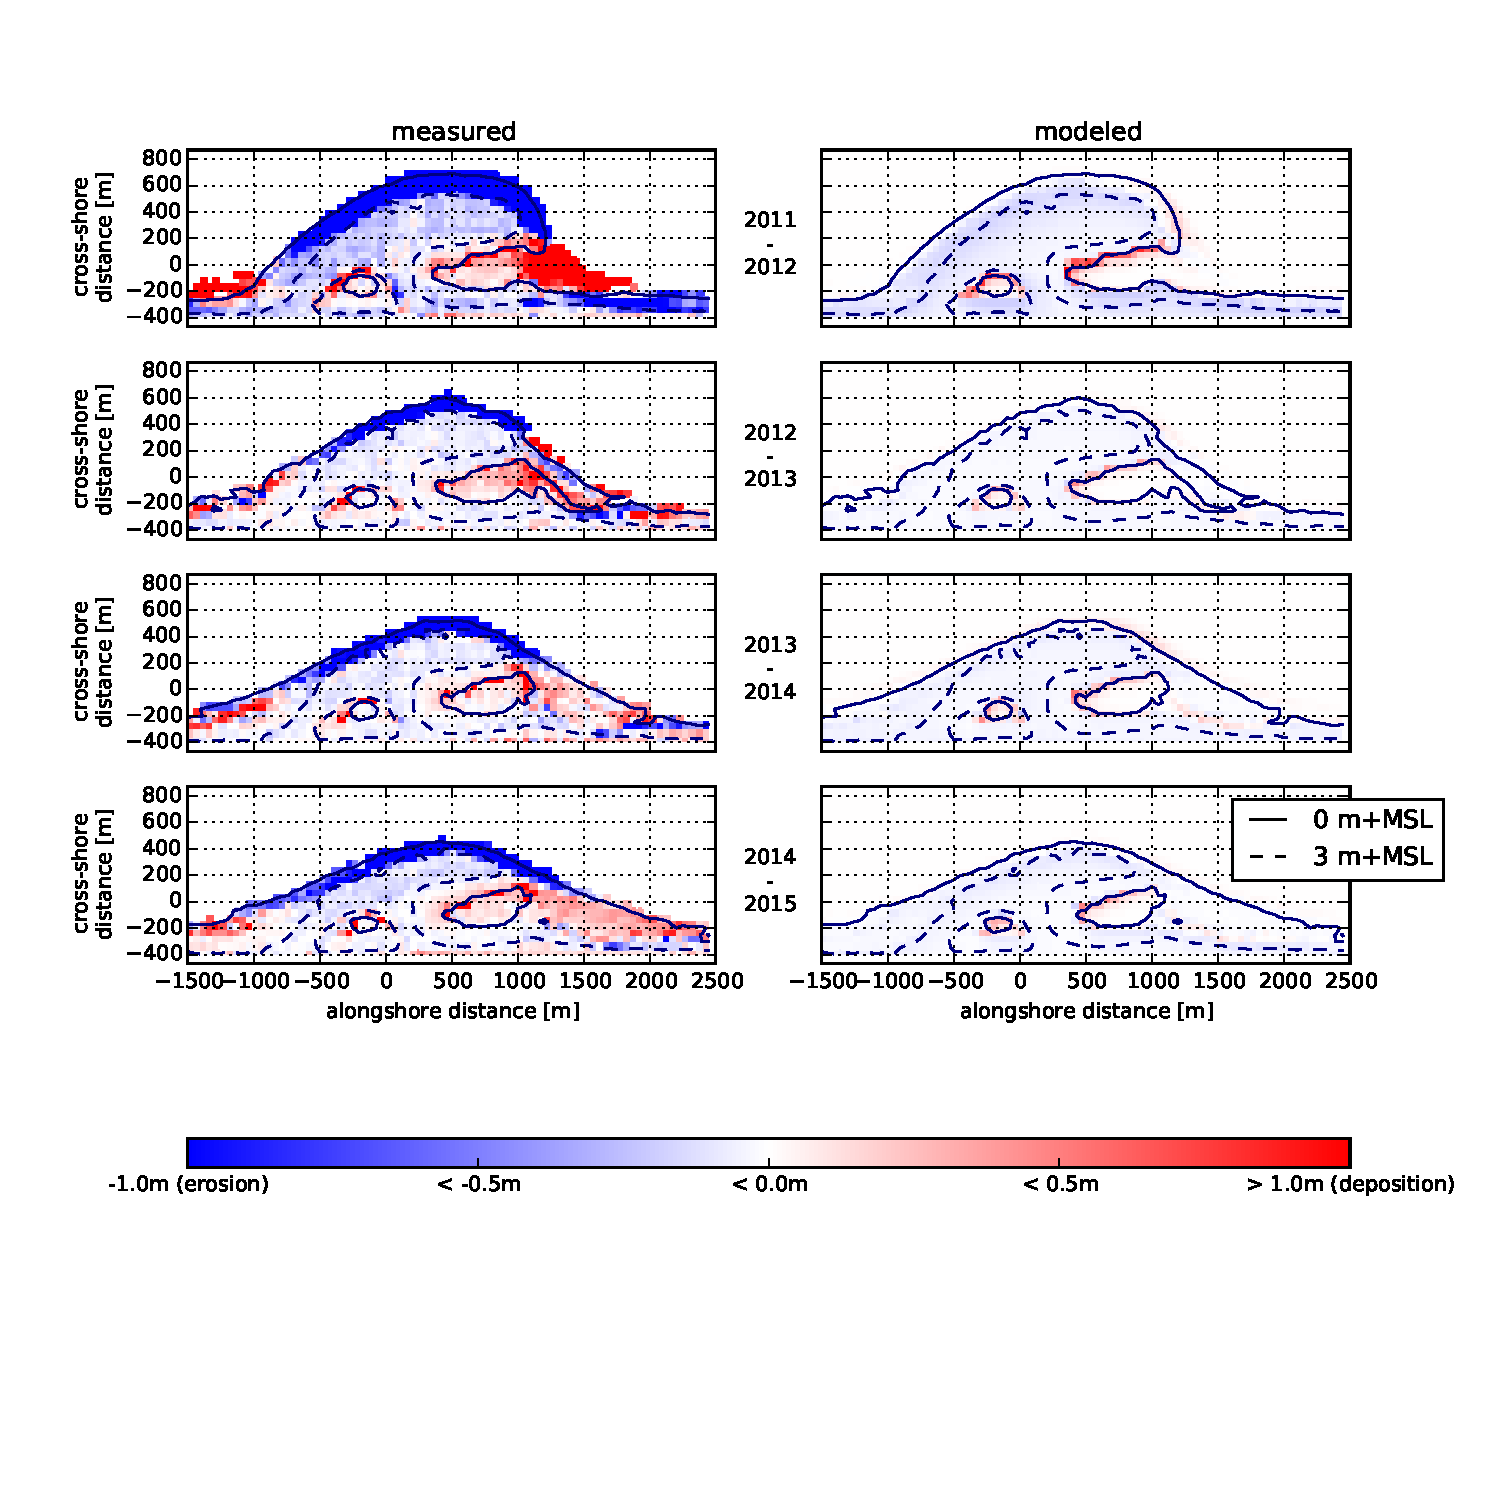
\includegraphics[width=\columnwidth]{../Figures/model_sedero}
  \caption{Measured and modeled yearly sedimentation and erosion
    above 0 m+MSL. Model results only include aeolian sediment
    transport as hydrodynamic sediment transport is not
    computed. Comparisons are made between the September surveys of
    each year.}
  \label{fig:sedero_model}
\end{figure}

\begin{figure}
  \centering
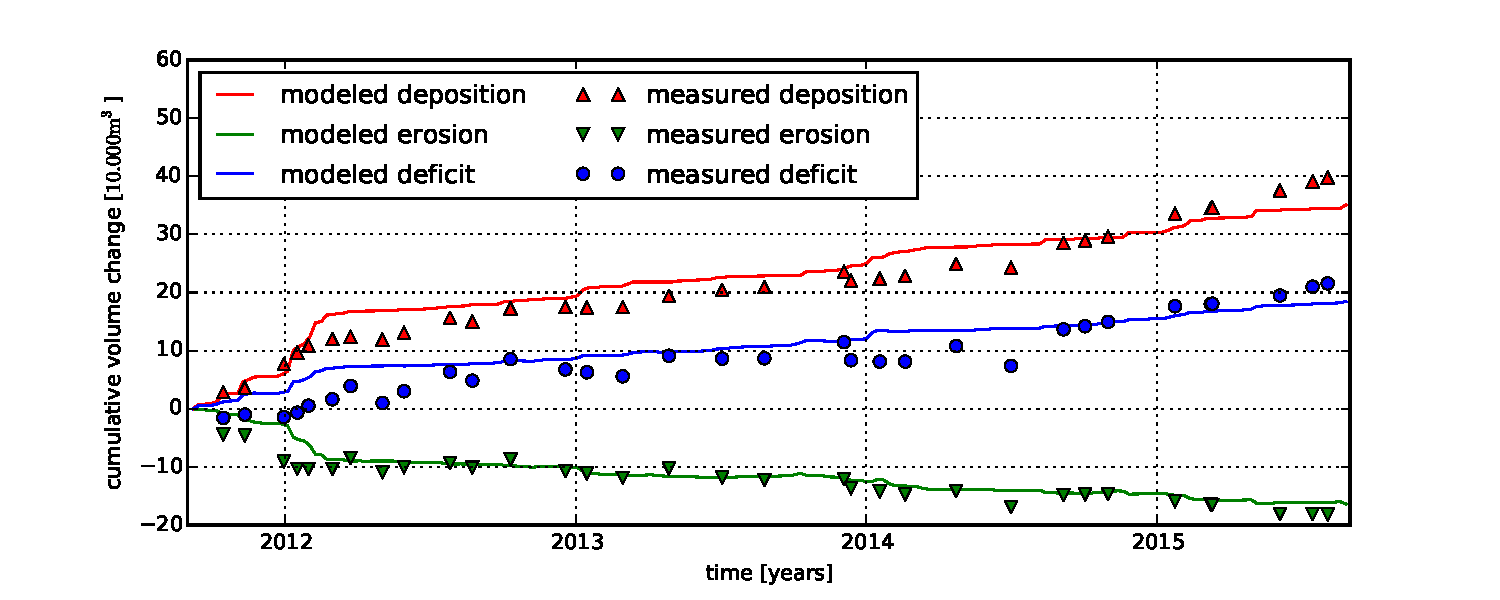
\includegraphics[width=\columnwidth]{../Figures/model_volumes_ts}
\caption{Measured and simulated net volume change of erosion and
  deposition volumes as presented in Figure
  \ref{fig:netvolumechange}.}
  \label{fig:netvolumechange_model}
\end{figure}

\begin{figure}
  \centering
  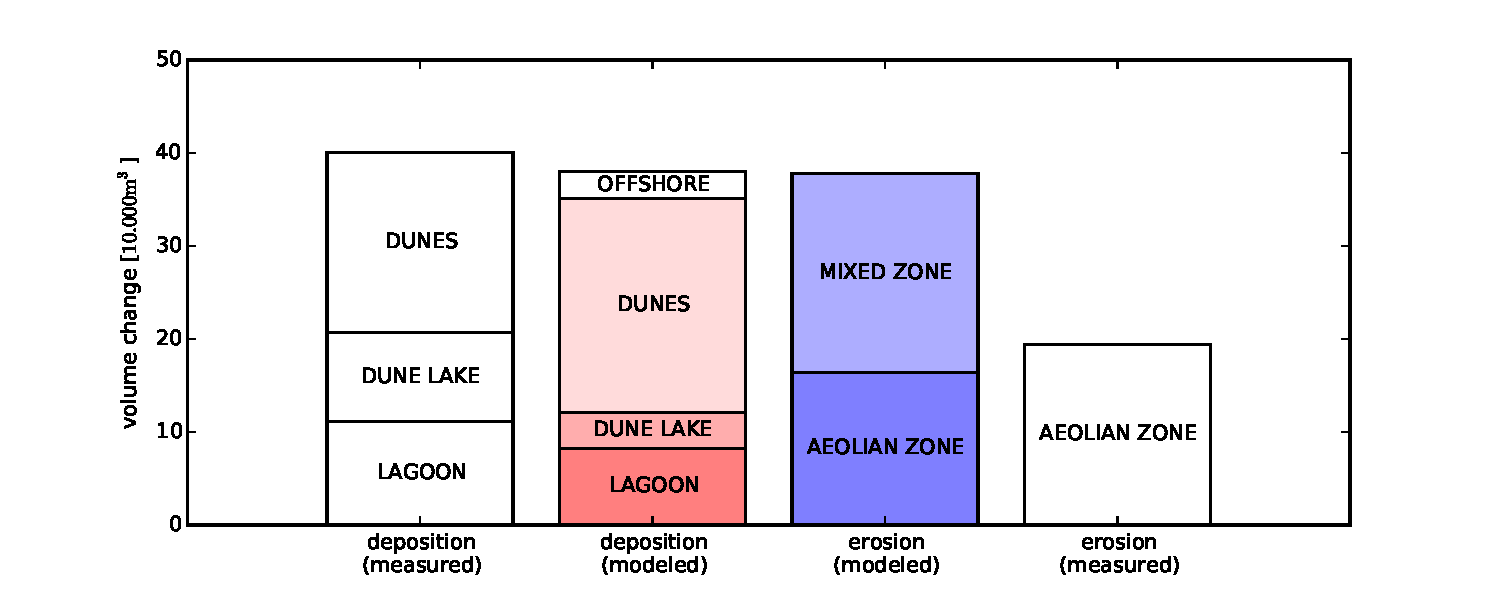
\includegraphics[width=\columnwidth]{../Figures/model_volumes}
  \caption{Total erosion and deposition volumes at the end of the
    simulation and measured total erosion and deposition volumes as
    presented in Figure \ref{fig:volumes_bars}.}
  \label{fig:volumes_bars_model}
\end{figure}

\begin{figure}
  \centering
  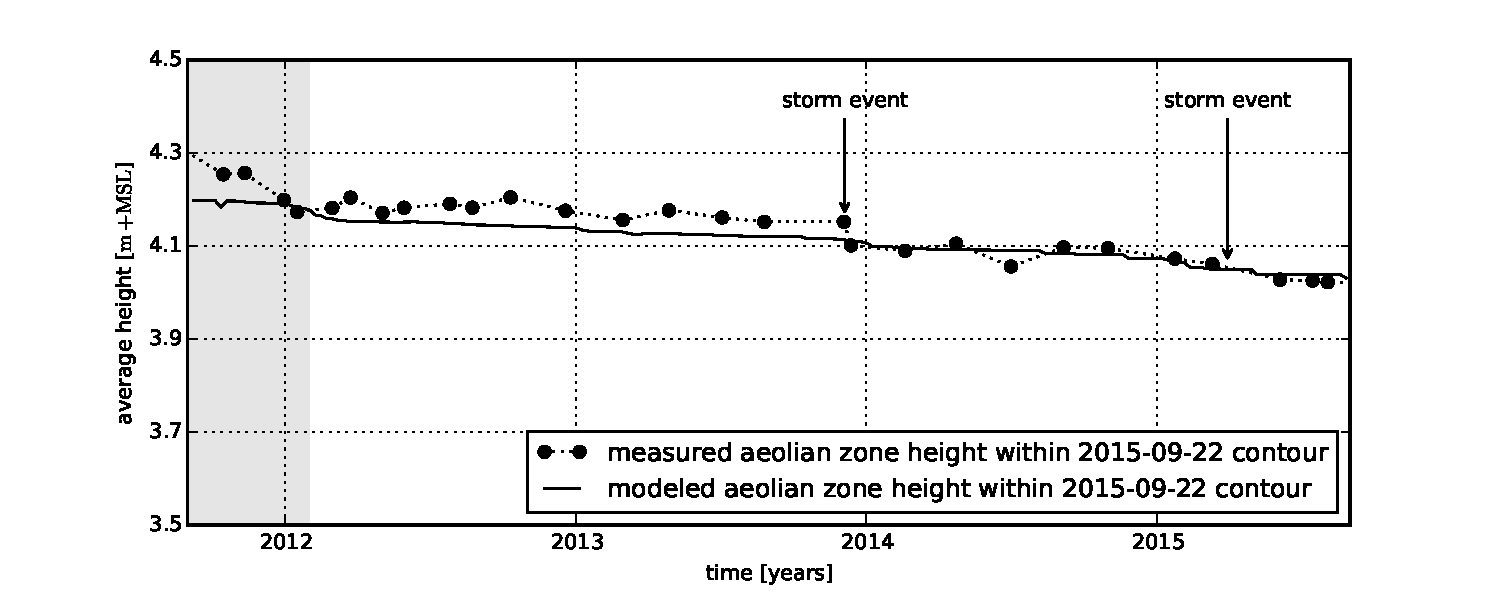
\includegraphics[width=\columnwidth]{../Figures/model_heights}
  \caption{Measured and simulated average beach height in the aeolian
    zone as presented in Figure \ref{fig:heights}.}
  \label{fig:heights_model}
\end{figure}

\begin{figure}
  \centering
  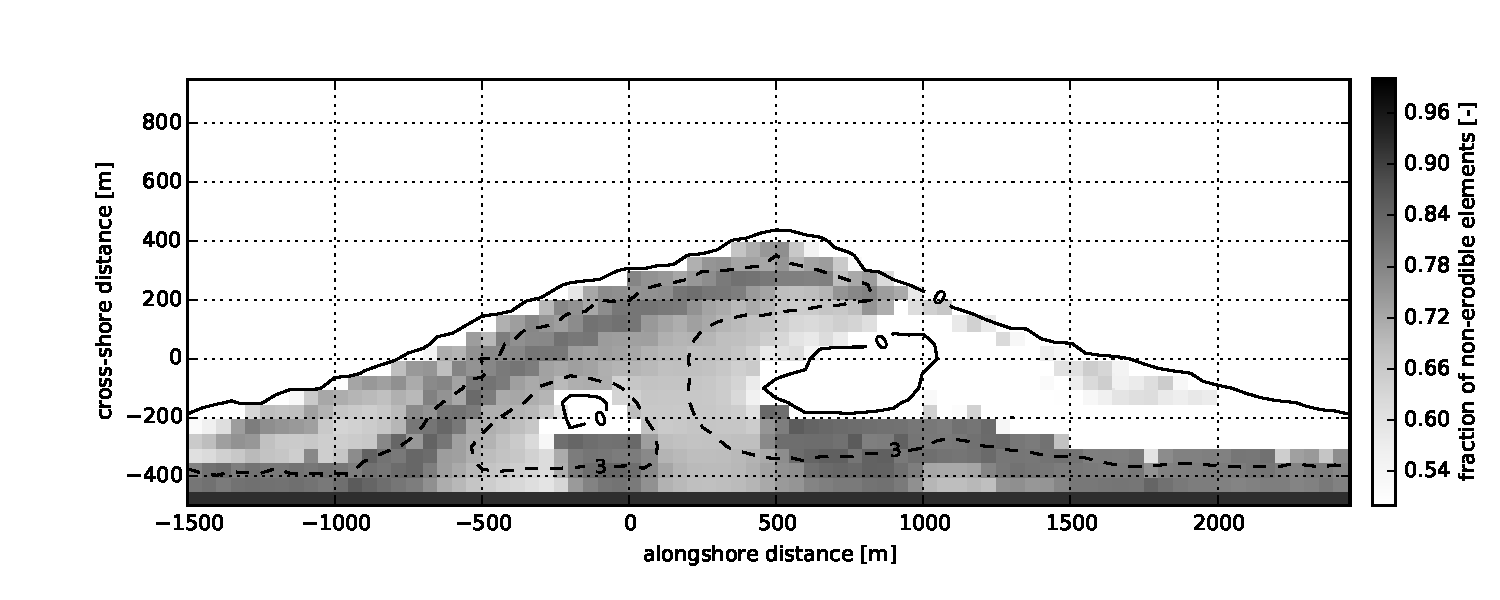
\includegraphics[width=\columnwidth]{../Figures/model_shellfraction}
  \caption{Simulated shell fraction in the aeolian zone at the end of
    the simulation.}
  \label{fig:shellfraction_model}
\end{figure}

Figure \ref{fig:sedero_model} shows that erosion from the aeolian zone
(Figure \ref{fig:decomposition2}, first row) is most pronounced in the
first year and least in the second year in both the measurements and
the model results. Also the deposition of aeolian sediment in the dune
lake and lagoon (Figure \ref{fig:decomposition2}, second row) is
observed in both the measurements and model results, although the
model underestimates these deposited volumes. The deposition in the
dune lake and lagoon is also more localized in the measurements than
in the model results. The spatial variability in the erosion of the
aeolian zone is larger in the measurements than in the model
results. The large variability measured in the mixed zone is not
present in the model results as hydrodynamic sediment transport is not
simulated.

The development of the total erosion and deposition volumes in the
Sand Motor domain in the four year period is represented well by the
model (Figure \ref{fig:netvolumechange_model}). The dune accumulation
volume is overestimated at the expense of the sediment volumes
deposited in the dune lake and lagoon (Figure
\ref{fig:volumes_bars_model}). As the dune area is not included in the
model domain, the sediment flux over the onshore boundary is assumed
to settle in the dunes entirely. The total sediment accumulation at
the end of the simulation is underestimated by 12\% as the offshore
sediment deposits are not included in the large scale sediment budget
analysis that are used for comparison. The underestimation is unique
for the last nine months of the simulation as the model overestimates
the total sediment accumulation with 5\% on average (Figure
\ref{fig:netvolumechange_model}). The relative importance of the mixed
zone as supplier of aeolian sediment is well captured. \mrq[hc]{1.3}

The change in beach height within the most recent 3 m+MSL contour,
that marks the aeolian zone, is represented by the model as the
$\mathrm{R^2}$ value is 0.71 and the RMSE is about 4 cm or 12\% of the
average bed level change (Figure \ref{fig:heights_model}). As the
change in beach height is computed within the most recent 3 m+MSL
contour, the discrepancy is illustrative for the differences in
spatial variability in erosion between measurements and model
results. The lowering of the beach in the aeolian zone in the first
half year of the simulation is particularly underestimated, while the
accelerated erosion in this period is well captured in the total
sediment transport. This indicates that sediment is eroded from
outside the most recent 3 m+MSL contour.

The coverage of non-erodible elements $\sigma \lambda$ [-] (Equation
\ref{eq:roughness_density}) in the aeolian zone varies between 60\%
and 80\% at the end of the simulation (Figure
\ref{fig:shellfraction_model}). The coverage is high compared to the
10\% -- 20\% shell coverage estimated to be present at the Sand Motor
above 3 m+MSL based on gridded photographs.
% (Figure \ref{fig:armoring}).

\begin{figure}
  \centering
  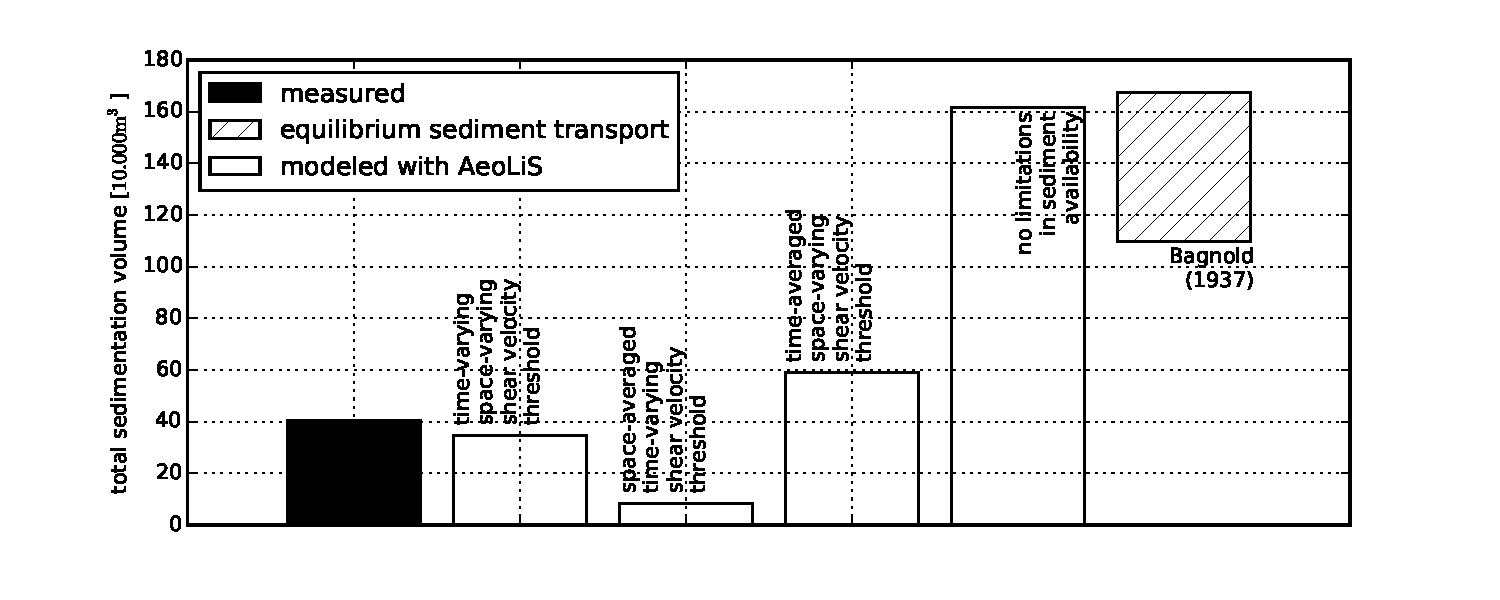
\includegraphics[width=\columnwidth]{../Figures/space_vs_time}
  \caption{The influence of time-varying and space-varying shear
    velocity thresholds on the total sedimentation volume. The two
    leftmost bars depict the measured and modeled sedimentation volume
    as obtained from the calibrated model (Figure
    \ref{fig:volumes_bars_model}). The middle two bars depict results
    from two separate model simulations in which a space-averaged
    threshold time series or a time-averaged threshold field is
    imposed respectively. The threshold averages are based on the
    result from the calibrated model. The two rightmost columns depict
    a result from a separate model simulation with a constant uniform
    threshold based on only a constant uniform median grain size and
    the estimated equilibrium sediment transport following
    \citet{Bagnold1937a} respectively (Table \ref{tab:models}).}
  \label{fig:space_vs_time}
\end{figure}

Both the spatial and temporal variations in aeolian sediment
availability are crucial for an accurate description of total
sedimentation and erosion volumes as well as an accurate prediction of
the aeolian sediment source and deposition areas. \mrq[hc]{4.3} Figure
\ref{fig:space_vs_time} compares the total sedimentation volume
according to measurements, the calibrated model and additional
simulations, that are variations of the calibrated model in which
spatial and/or temporal variations in the shear velocity threshold are
averaged out. During these additional simulations the shear velocity
threshold is not computed by the model, but space- and/or
time-averaged thresholds based on the model results of the calibrated
model are imposed. Negligence of the spatial variations results in a
79\% underestimation of the total sedimentation volume and a relative
contribution of 8\% of the mixed zones. The negligence of the temporal
variations results in a 46\% overestimation of the total sedimentation
volume and a relative contribution of 86\% of the mixed zones.  In
addition, a simulation without limitations in sediment availability
overestimates the measured total sedimentation volumes with 400\%,
which is comparable to the wind transport capacity following
\citet[][Figure \ref{fig:models}]{Bagnold1937a}.

% R^2

% distribution between areas

% beach height

% shell coverage

% runup not taken into account

%\begin{figure}
%  \centering
%\includegraphics[width=\columnwidth]{../Figures/volumes_ts_forecast}
%\caption{Measured and simulated net volume change of erosion and
%  deposition volumes for the period September 1, 2015 to September 1,
%  2016 that was not included in the model calibration.}
%  \label{fig:netvolumechange_model2}
%\end{figure}
%
%The comparison of measurements and model results for the period
% between September 1, 2011 and September 1, 2015 illustrates the
% descriptive capabilities of the model. Figure
% \ref{fig:netvolumechange_model2} shows the measured and modeled
% volume change between September 1, 2015 and September 1, 2016. The
% continuation of the total sediment accumulation is predicted [TODO],
% given the $\mathrm{R^2}$ of [TODO] and RMSE of
% [TODO]\%.

\section{Discussion}

The model results show that multi-annual aeolian sediment erosion and
deposition volumes, and the relative importance of the mixed zones as
source of aeolian sediment are reproduced with reasonable
accuracy. This suggests that indeed significant limitations in
sediment availability, due to soil moisture content and beach
armoring, govern aeolian sediment transport in the Sand Motor domain.
A comparison with a simulation without limitation in sediment
availability suggests that aeolian sediment availability in the Sand
Motor domain is limited to about 25\% -- 35\% of the wind transport
capacity.

The negligence of spatial variations causes the model to underestimate
the measured total sedimentation volume. The sediment supply from the
relatively small mixed zone is marginalized as the imposed
space-averaged shear velocity threshold is relatively high. In
contrast, the negligence of temporal variations causes the model to
overestimate the measured total sedimentation volume. The sediment
supply from the mixed zones is increased as the effect of its periodic
flooding is averaged out. At the same time, the sediment supply from
the aeolian zone is decreased as the influence of beach armoring
affects sediment availability from the start of the simulation rather
than after the development of the beach armor layer. Therefore, the
total sedimentation volume is not only overestimated, but also the
importance of the mixed zones as supplier of aeolian sediment.

\subsection{Seasonal and local variations in sedimentation and
  erosion}

% advection assumption / diffusion / gusts
%The advection equation in combination with a diffusive numerical
%scheme results in smooth solutions. Small-scale variability in erosion
%and deposition are therefore not described by the model. Besides,
%measured local variations are likely promoted by local variations in
%initial topography and bed composition that also induce local
%variations in wind shear. These initial variations are not taken into
%account in the simulations.

The model can reproduce multi-annual trends in sedimentation volume,
which is the aim of the hindcast, but seasonal and local variations
are sometimes not represented by the model. An analysis of these
variations is interesting as they influence the accuracy of specific
model results.

Average wind speeds tend to be elevated in December and January
(Figure \ref{fig:boundaryconditions}), which leads to short periods of
accelerated sediment accumulation in the beginning of 2012, 2013 and
2015 that are captured well by the model. Early 2014 no accelerated
sediment accumulation is measured, while the model simulation shows an
increase in sediment accumulation originating from the mixed zones
similar to other years.

The discrepancy early 2014 might be explained by topographic changes
induced by hydrodynamic forces. On December 5th, 2013 an exceptional
storm hit the Dutch coast. During this storm a significant decrease in
aeolian deposits in the lagoon was observed, while deposits in the
dunes and dune lake increased only marginally. The assumption that the
closed end of the lagoon is mainly governed by aeolian sediment
transport might be violated in these exceptional conditions. At the
same time, the erosion of the aeolian zone that day equaled the total
erosion of the aeolian zone that year. Consequently, the total
subaerial sediment volume decreased that day with about
$\mathrm{1 \cdot 10^4}$ $\mathrm{m^3}$, possibly caused by
hydrodynamic forces. This suggests that the simplified hydrodynamics,
despite the use of a hydrodynamic mask, are a limiting factor in
describing the Sand Motor's subaerial morphodynamics during extreme
storms.

In the first months of the simulation, the total sediment accumulation
is well represented, but erosion of the aeolian zone is
underestimated. As beach armoring is the most important availability
limitation in the aeolian zone, this suggests that the armoring rate
is overestimated by the model. The armoring rate is mainly influenced
by initial shell fraction of 5\%, which might be
overestimated. Alternatively, the initially uniform distribution of
shells in the bed is not an accurate representation of reality.

Measured erosion and deposition rates exceed modeled erosion and
deposition rates in the final nine months of the simulation. In this
period dune growth seems to accelerate, while neither the deposition
in the dune lake and lagoon did accelerate nor did the wind speed
increase. The apparent acceleration is therefore solely found in the
half yearly lidar measurements of the dune area \citep{Hoonhout2017a}
and is consequently based on a single data point. Despite the
uncertainty involved in the measured acceleration, also precipitation
rates, that were up to 70\% lower in this period compared to the same
period in other years, might explain the discrepancy at the end of the
simulation \citep{Jackson1998}. For the hindcast no precipitation time
series are imposed as the effect on the aeolian sediment transport
rate is not properly understood yet. Consequently, the calibration of
the model might have resulted in an overestimated importance of beach
armoring to compensate for the negligence of precipitation.

% morphological feedback
The distribution of the aeolian sediment deposits over the dune lake,
lagoon and dunes is not represented well as deposits in the dune lake
and lagoon are underestimated. Additional hydrodynamic and hydrologic
processes, like wind setup and groundwater seepage, might cause the
entrapment area in reality to be larger than modeled. But more
importantly, the dune lake and lagoon are positioned in the lee of the
Sand Motor crest with respect to the predominant southwesterly wind
direction. The height difference between the Sand Motor crest and the
water level in the lagoon and dune lake is several meters, which is
likely to influence the local wind field significantly. The probable
decrease in wind shear in the lee of the Sand Motor crest promotes
deposition of aeolian sediment and likely hampers supply to the
dunes. These local variations in wind shear are not included in the
simulations.

\subsection{Beach armoring, sediment availability and the shear
  velocity threshold}

% As the $\sigma$ value is an optimal average for the entire model
% domain and duration it can be questioned if an incidental increase
% in soil moisture due to precipitation can influence sediment supply
% significantly.

\begin{figure}
  \centering
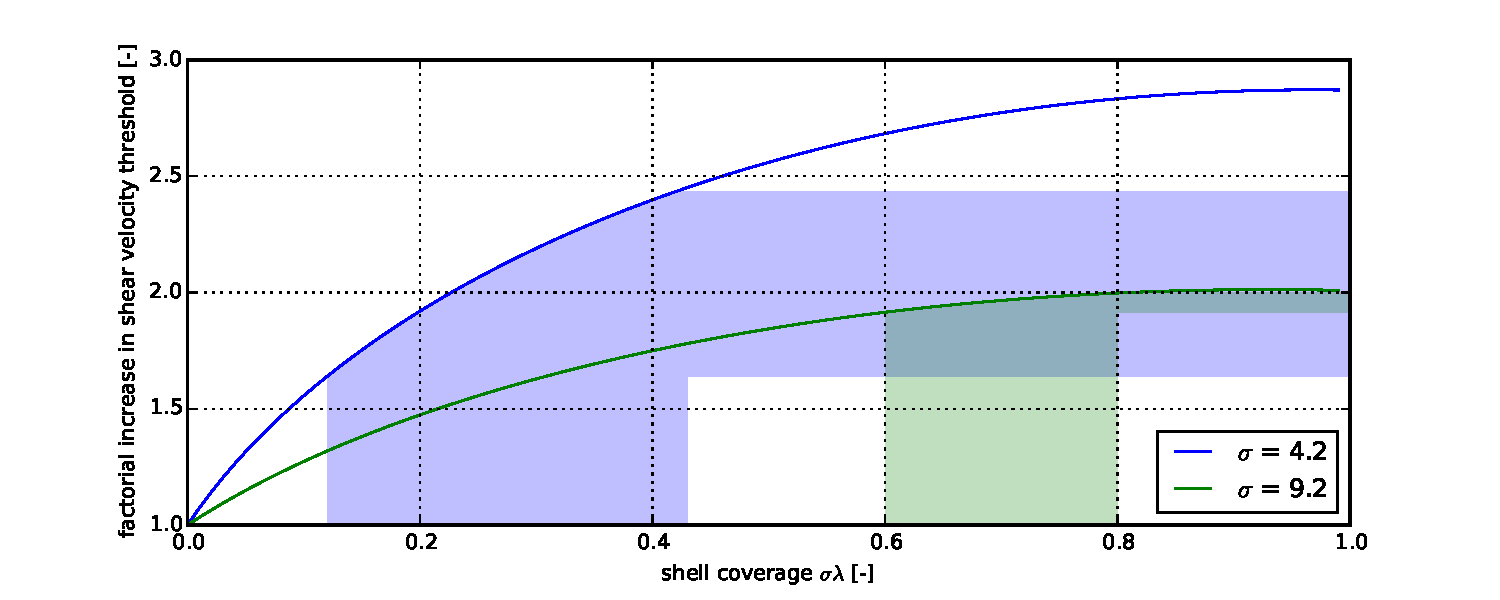
\includegraphics[width=\columnwidth]{../Figures/sigma}
\caption{Relation between shear velocity threshold, shell coverage and
  $\sigma$ according to \citet[][Equation
  \ref{eq:raupach2}]{Raupach1993}. The shaded areas indicate the
  relevant parameter ranges from \citet{McKennaNeuman2012} (blue) and
  the model results (green).}
  \label{fig:sigma}
\end{figure}

The influence of beach armoring is reflected in the model by both
$\sigma$ and the roughness density $\lambda$ (Equation
\ref{eq:raupach2} and \ref{eq:roughness_density}). The optimal value
for $\sigma$ was found to be 9.2, which is high compared to the value
of 4.2 found by \citet{McKennaNeuman2012}. The difference suggests
that the roughness elements at the Sand Motor protrude less from the
bed compared to what was found in the wind tunnel
experiments. Consequently, the importance of beach armoring would be
relatively low at the Sand Motor. However, the low $\sigma$ value is
largely compensated by the roughness density $\lambda$ reflected in a
shell coverage $\sigma \lambda$ that is high compared to what was
found in the wind tunnel experiments (12\% -- 43\% on average) and
what is found at the Sand Motor field site (10\% -- 20\%). Figure
\ref{fig:sigma} shows that the combination of high shell coverage and
$\sigma$ value results in a very similar increase of the shear
velocity threshold compared to the wind tunnel experiments presented
by \citet{McKennaNeuman2012}.

The reason that the model calibration resulted in this particular
value for $\sigma$ is that the model does not differentiate between
the fluid and impact velocity threshold.  Therefore, the roughness
elements in the model affect the initiation of sediment transport
equal to the continuation of sediment transport. The potential
reduction in sediment availability increases with a decreasing value
for $\sigma$ (if $m$ = 0.5, Figure \ref{fig:sigma}) and is implemented
through an increase in shear velocity threshold. The shear velocity
threshold also affects aeolian sediment already in transport and
originating from upwind, unarmored beach areas, like the mixed
zones. Sediments from upwind areas are therefore partially deposited
in the aeolian zone as soon a beach armor layer develops. For low
values for $\sigma$ the local deposition of sediment from upwind areas
is already significant with low shell coverage. Low $\sigma$ values
therefore reduce the total sediment accumulation in the dunes
quickly. In order for the model to provide reasonable total sediment
transport rates, a higher value for $\sigma$ was found in the
calibration that ultimately induces a higher shell coverage. The value
for $\sigma$ therefore does not only represent a spatiotemporal
averaged emergence of roughness elements, but also a compromise
between its effect on the fluid and impact velocity threshold.
%The
%implementation of roughness elements in the model can explain the high
%value for $\sigma$, but it particularly illustrates the necessity to
%differentiate between initiation and continuation.% of motion as
%observed in recent laboratory measurements (REFS RALEIGH MARTIN).
% associated with the fluid and impact velocity threshold respectively.

%\subsection{Predictive capabilities of the model}
%
%The period from September 1, 2015 to September 1, 2016 was not
% included in the calibration. Simulation of the total sediment
% accumulation in this period therefore provides insight in the
% predictive capabilities of the calibrated model. The
% $\mathrm{R}^2$ and RMSE values suggests that the model
% has both descriptive and predictive capabilities.




% average wind vs gusts

% wind field

% bed composition layers

% offshore deposits

% salt crusts

% distinction between thresholds for entrainment and continuation

\section{Conclusions}

The Sand Motor hindcast shows that the reduction of aeolian sediment
availability due to soil moisture and beach armoring can largely
explain the low accumulation volumes in the Sand Motor domain. The
\textsc{AeoLiS} model has shown to be quantitatively valuable and
practically applicable. The model provides a framework for the
description of complex spatiotemporal variations in aeolian sediment
availability and its relation to sediment transport that has not yet
been exploited in full.

\bigskip

\noindent From the hindcast the following conclusions can be drawn:

\begin{itemize}
\item The \textsc{AeoLiS} model is able to reproduce multi-annual
  aeolian sediment transport rates in the Sand Motor domain in the
  four years after its construction with a RMSE of
  $3 \cdot 10^4 ~ \mathrm{m^3}$ and $\mathrm{R^2}$ of 0.92 when time
  series of measured and modeled total aeolian sediment transport
  volumes are compared.
\item The \textsc{AeoLiS} model is able to reproduce large scale
  spatial patterns in aeolian sediment transport in the Sand Motor
  domain in the four years after its construction, but underestimates
  the deposition in the dune lake and lagoon.
\item The \textsc{AeoLiS} model overestimates the total sedimentation
  volume with 5\% on average, but underestimates the total
  sedimentation volume with 12\% at the end of the simulation. The
  discrepancy at the end of the simulation might be caused by a
  particularly dry season as precipitation is not included in the
  simulations.
  % \item The \textsc{AeoLiS} model has predictive capabilities as the
  %   calibrated model describes new period of measurements with a
  %   RMSE of XX\% and $\mathrm{R}^2$ of 0.XX.
\item The \textsc{AeoLiS} model is able to capture the seasonal
  variations in sediment transport in all years, except for early 2014
  when significant morphological change is possibly related to
  hydrodynamic sediment transport that is not included in the
  simulations.
\item The \textsc{AeoLiS} model overestimates the shell coverage,
  which compensates the high value for $\sigma$. The high $\sigma$
  value is a compromise between the fluid and impact threshold that
  are currently assumed to be equal.
\item The combination of spatial and temporal variations in aeolian
  sediment availability, due to the combined influence of soil
  moisture, sediment sorting and beach armoring, and the feedback
  between aeolian sediment availability and transport is essential for
  an accurate estimate of the total sedimentation volume and the
  corresponding aeolian sediment source areas in the Sand Motor
  domain.
\end{itemize}

%%% Local Variables:
%%% mode: latex
%%% TeX-master: "thesis"
%%% End:
